%! suppress = TooLargeSection
%! suppress = MissingLabel
\documentclass[letterpaper,12pt,sfdefaults=false]{scrreprt}
\usepackage{latex/packages}
% Basics + Fonts
\RequirePackage{etex}
\RequirePackage{xspace}
\RequirePackage{fontawesome5}
\RequirePackage[verbose]{newunicodechar}
\RequirePackage{sansmath}
% Document
\RequirePackage[bottom]{footmisc}
\RequirePackage{filecontents}
\RequirePackage{pdfpages}
\RequirePackage{color}
\RequirePackage{adjustbox}
\RequirePackage[inline]{enumitem}
\RequirePackage{fnpct}
\RequirePackage{imakeidx}
\RequirePackage[setpagesize=false]{hyperref} % FIX! https://tex.stackexchange.com/a/28800/
\RequirePackage[acronym,nomain,section=chapter,numberedsection=autolabel,nogroupskip]{glossaries}
\RequirePackage{glossary-longragged}
\RequirePackage{mdframed}
% Math
\RequirePackage{amsmath}
\RequirePackage{mathtools}
\RequirePackage{amssymb}
\RequirePackage{amsfonts}
\RequirePackage{amsthm}
\RequirePackage{ebproof}
\RequirePackage{nicematrix}
\RequirePackage[theorems,breakable,hooks,most]{tcolorbox}
\RequirePackage{cases}
\RequirePackage{stmaryrd}
%\RequirePackage{bm}
% Tables + figures
\RequirePackage{tabularx}
\RequirePackage{ltablex}
\RequirePackage{multicol}
\RequirePackage{multirow}
\RequirePackage{caption}
\RequirePackage{subcaption}
\RequirePackage{tikz}
% Code + algorithms
\RequirePackage{algorithm}
\RequirePackage{algorithmicx}
\RequirePackage[noend]{algpseudocode}
%! suppress = FileNotFound
\RequirePackage{ottalt}

\usepackage{everypage,pdfpages,eso-pic}
\usepackage[yyyymmdd,24hr]{datetime}
\renewcommand{\dateseparator}{-}
\def\PageTopMargin{1in}
\def\PageLeftMargin{2.2in}
\newcommand\atxy[3]{%
\AddEverypageHook{\smash{\hspace*{\dimexpr-\PageLeftMargin-\hoffset+#1\relax}%
\raisebox{\dimexpr\PageTopMargin+\voffset-#2\relax}{#3}}}}
\atxy{\dimexpr1.5in}{0.1in}{%
\raisebox{-\height}{\small\normalfont\sffamily{compiled: {\yyyymmdddate\today} \currenttime}}}
\usepackage[pagewise]{lineno}
\renewcommand{\linenumberfont}{\normalfont\sffamily\tiny\color{red}}
\AtBeginDocument{\linenumbers}

%%%%%%%%%%%%%%%%%%%%%%%%%%%%%%%%%%%%%%%%%%%%%%%%%%%%%%%%%%%%%%%%%%%%%%%%%%%%%%%%
% GUIDES
% https://guides.augusta.edu/etd
% https://augustauniversity.app.box.com/s/vj0ygpy8tvyqmsbae8y0qp9767ta7jb9

\date{\today}
\title{On Practical Realization of Implicit Computational Complexity}
\author{Neea Rusch}
\newcommand\mykeywords{%
{programming languages}, %
{static program analysis}, %
{implicit computational complexity}, %
{verification}, %
{formal methods}}

\makeatletter
\hypersetup{
  pdftitle={{\@title}},
  pdfauthor={{\@author}},
  pdfkeywords={\mykeywords},
  pdfsubject={PhD Dissertation},
  bookmarks=true,
  unicode=false,
  pdftoolbar=true,
  pdfmenubar=true,
  pdffitwindow=false,
  pdfstartview={FitH},
  pdfnewwindow=true,
  ocgcolorlinks}
\makeatother

\newcommand\CTNT{Cl{\'{e}}ment Aubert, Thomas Rubiano, Neea Rusch, Thomas Seiller}
%%%%%%%%%%%%%%%%%%%%%%%%%%%%%%%%%%%%%%%%%%%%%%%%%%%%%%%%%%%%%%%%%%%%%%%%%%%%%%%%
\begin{document}
\pagenumbering{arabic}
\thispagestyle{empty}
\AddToHookNext{shipout/foreground}{\put (0, 0)%
{\pdfbookmark[0]{Cover}{sec:cover}}}
\label{sec:cover}\maketitle\clearpage
\thispagestyle{empty}
\AddToHookNext{shipout/foreground}{\put (0, 0)%
{\pdfbookmark[0]{Acknowledgements}{sec:acks}}}
\section*{Acknowledgements}
\label{sec:acks}
acknowledgements

% Acknowledgements – include a detailed summary of the work performed by other
% authors on published or accepted manuscripts used in the thesis/dissertation,
% if applicable.\clearpage
\thispagestyle{empty}
\AddToHookNext{shipout/foreground}{\put (0, 0)%
{\pdfbookmark[0]{Abstract}{sec:abstract}}}
\section*{\uppercase{Abstract}}
\label{sec:abstract}

\noindent{\MakeUppercase \ETDAUTHOR}

\noindent\ETDTITLE

\noindent(Under the direction of {\MakeUppercase \ETDADVISOR})

% The text of abstract then begins three lines after the title, and is double-spaced.
\vspace{2em}
\noindentThe abstract must not exceed 350 words.
The abstract consists of a succinct summary of the thesis/dissertation and the conclusions reached.
Opinions should be omitted.

\vspace{2em}
% The words must be listed three lines below the body of the abstract,
\noindent <insert a list of keywords>\clearpage
\pdfbookmark[0]{\contentsname}{toc}
\pagestyle{empty}\tableofcontents\clearpage
\pdfbookmark[0]{\listtablename}{lot}\listoftables\clearpage
\pdfbookmark[0]{\listfigurename}{lof}\listoffigures\clearpage

%-------------------------------------------------------------------------------
%	1. INTRODUCTION
%-------------------------------------------------------------------------------
\setcounter{chapter}{0}
\chapter{Introduction}\label{ch:introduction}
\clearpage\section{Problem statement}\label{sec:intro}

Statement of the problem and specific aims of the overall project.


\clearpage\section{Preliminaries}\label{sec:pre}

Literature review and discussion of the rationale of the project.

It is expected that the literature review will be more comprehensive than
those presented in the included publications.



%-------------------------------------------------------------------------------
%	2. PUBLISHED MANUSCRIPTS
%-------------------------------------------------------------------------------
\chapter{Published Manuscripts}\label{ch:published-manuscripts}\clearpage

\section{pymwp: A Static Analyzer Determining Polynomial Growth Bounds}\label{sec:atva}
\ainfoX{\CTNT}{\href{https://atva-conference.org/2023}
{International Symposium on Automated Technology for Verification and Analysis, 2023}}
{\noindent Software artifact:
\href{https://doi.org/10.5281/zenodo.7908484}{10.5281/zenodo.7908484}
\newline\noindent Tool user guide: \aref{app:sec:tool-guide}}
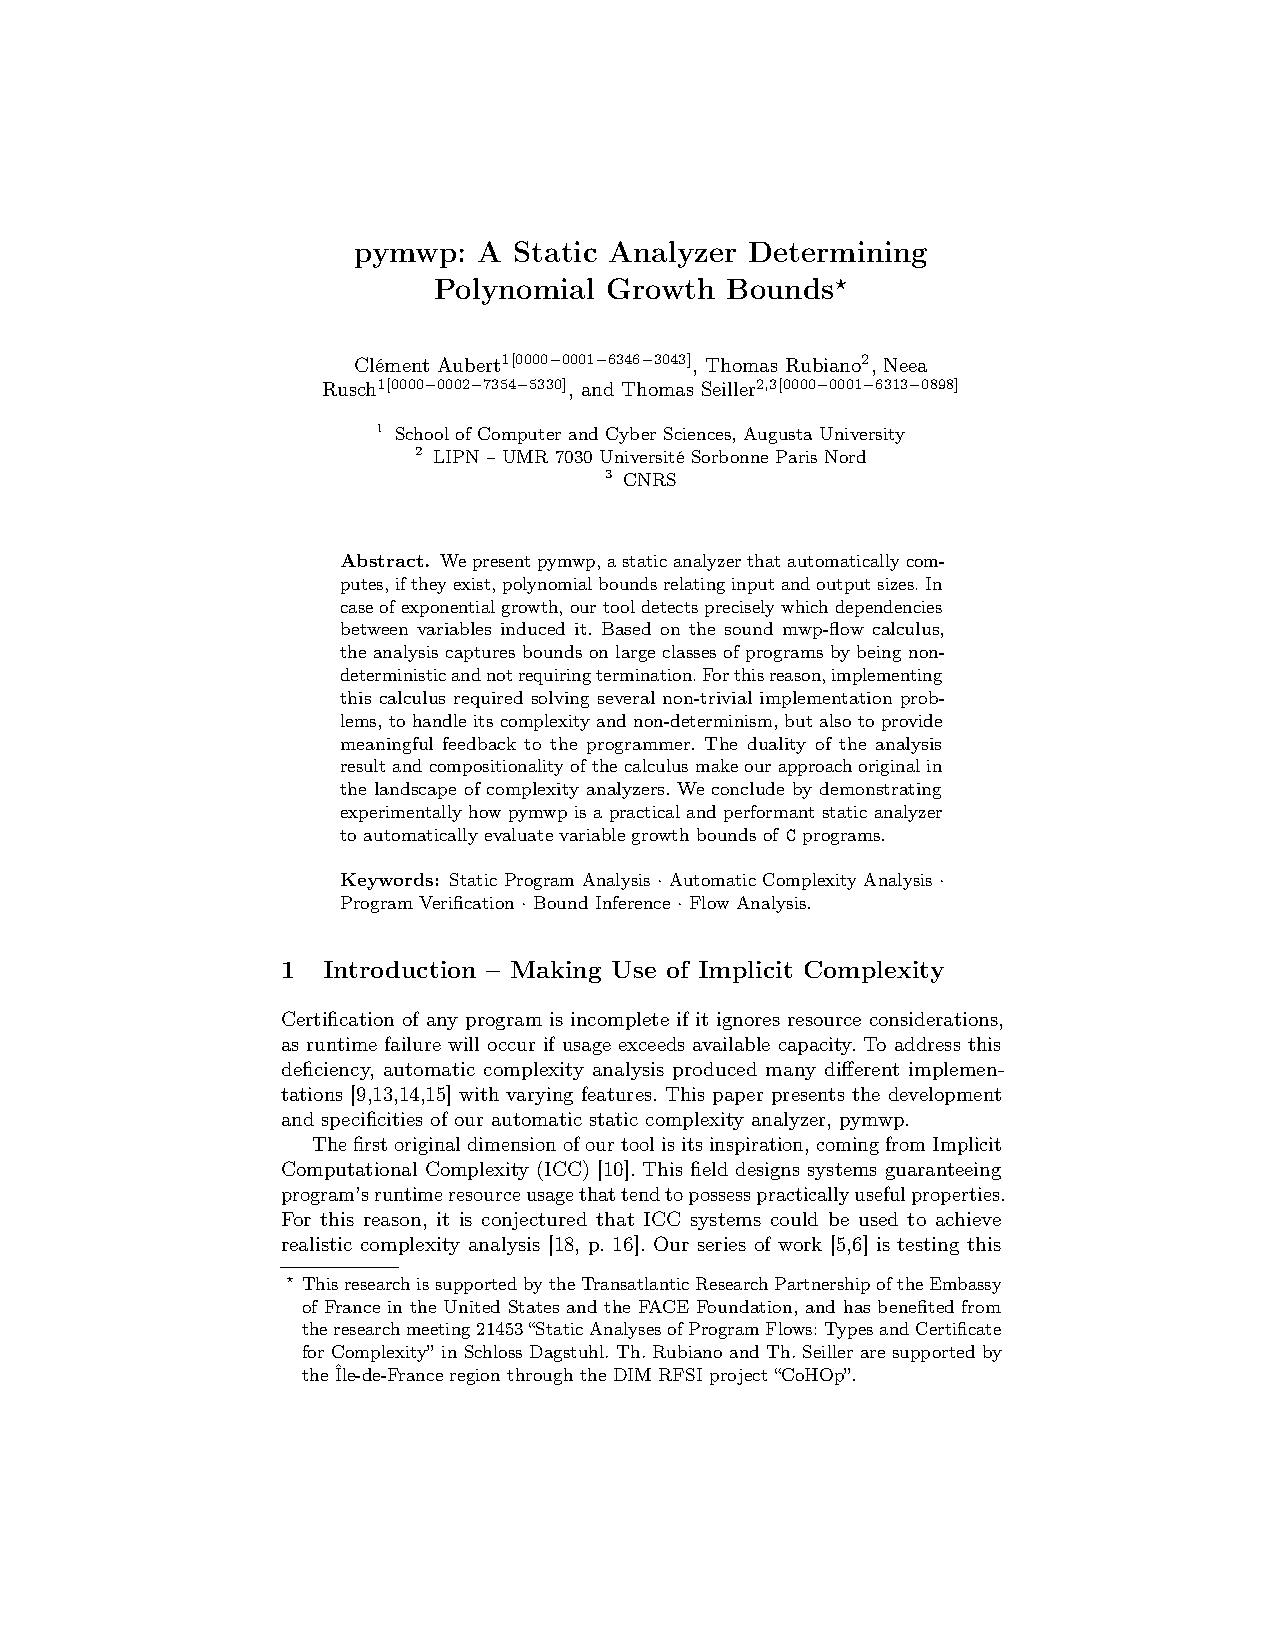
\includepdf[pages={1-},
addtotoc={
   1,subsection,2,{Introduction -- Making Use of Implicit Complexity},sec:intro,
   3,subsection,2,{Calculating Bounds with \mwp-Analysis},sec:idea,
   5,subsection,2,{Technical Overview of pymwp},sec:tool,
   6,subsection,2,{Implementation Advancements},sec:solutions,
   8,subsection,2,{Experimental Evaluation},sec:eval,
  11,subsection,2,{Conclusion},sec:conc},
addtolist={
5,table,Comparison of obtained resource bounds,tab:compare,
10,table,Benchmark results,tab:eval,
10,table,Examples of obtained bounds,tab:bounds},
pagecommand={\thispagestyle{empty}%
\addtoindex{pymwp}{1}
\addtoindex{pymwp}{2}
\addtoindex{pymwp}{4}
\addtoindex{pymwp}{5}
\addtoindex{pymwp}{6}
\addtoindex{pymwp}{7}
\addtoindex{pymwp}{8}
\addtoindex{pymwp}{9}
\addtoindex{pymwp}{11}
\addtoindex{LOOPUS}{4}
\addtoindex{LOOPUS}{5}
\addtoindex{C4B}{4}
\addtoindex{C4B}{5}
\addtoindex{pycparser}{6}
\addtoindex{mwp-bound}{3}
\addtoindex{mwp-bound}{8}
}]{papers/atva/main.pdf}

%-------------------------------------------------------------------------------
%	3. UNPUBLISHED RESEARCH
%-------------------------------------------------------------------------------
\chapter{Unpublished Research}\label{ch:unpublished-research}\clearpage
% This can include manuscripts, in the journal format, that have been submitted
% forpublication that are under review at the time of dissertation submission.
% Manuscripts that have been rejected or that have not been submitted (in
% preparation) cannot be included in the journal format (i.e. must conform to
% the traditional dissertation format). For manuscripts that have been
% submitted and are under review, the first authorship of the candidate must be
% maintained when the manuscript is published.

\section{An Information Flow Calculus for Non-Interference}\label{sec:ni-analysis}
\ainfoX{Cl{\'{e}}ment Aubert, Neea Rusch}
{\href{https://plas24.github.io}
{The 19th Workshop on Programming Languages and Analysis for Security, 2024}}
{\abspage{Sensitive data exposure is persistently ranked among the top-ten web application security risks, thus every software developer should actively combat data exposure vulnerabilities.
Information flow controls offer mechanisms to enforce data confidentiality.
Unfortunately, strict controls are too restrictive for real applications and innovation is needed to obtain practical solutions.
We present a brave new idea: an information flow calculus for non-interference.
Our formulation enforces that command composition does not create nor erase non-interference violations, and the sound calculus pinpoints precisely where violations occur.
The calculus can be implemented as an automatic, compositional, and annotation-free static security analyzer to obtain confidentiality guarantees in practice.}}
\subsection{Introduction}
\label{plas-introduction}

%\neea{Introduce non-interference and why we care about it.}
Careless exposure of sensitive information is at the core of numerous modern software security vulnerabilities and exploits.
Access control, firewalls, and encryption are among the control mechanisms to enforce \emph{confidentiality}, \ie disclosure of information to  authorized parties only.
Unfortunately, those controls are insufficient to provide end-to-end guarantees, since confidentiality is not ensured once information has been used as input data to a program~\cite{zdancewic2004}.
\emph{Non-interference}~\cite{goguen1982} is a classical program security property, that constrains information flow during computation.
A program is non-interfering when secret data does not affect calculation of public outputs~\cite{sabelfeld2003}.

%\neea{Explain why NI is interesting problem and requires more exploration, despite existing works.}
Although non-interference is a desirable property, it is in general undecidable by Rice's Theorem~\cite{rice1953}. %, determining if a program is non-interfering is undecidable.
Instead, various approximative approaches have emerged to reason about non-interference in theory~\cite{VolpanoI1996,abadi1999b,bowman2015} and practice~\cite{Myers1999,hammer2009,Broberg2013,arzt2014,huang2014}.
In this work, we focus on \emph{language-based security},
a family of techniques founded on programming languages principles \eg semantics, analysis, type systems, and rewriting;
as information-flow controls for enforcing non-interference~\cite{schneider2001,sabelfeld2003}.
A well-established technique %convention 
is using a security type system that insures non-interference via type-checking at compile-time.
% , where non-interference is established efficiently by type-checking at compile-time.

%\neea{Clearly identify and state the main idea, include novelty, and why useful}
In this work we take a different approach by presenting an \emph{information flow calculus} for non-interference.
It is an automatable, fully-static analysis of imperative program syntax, for deriving the semantic property of non-interference.
The technique is adapted from prior work~\cite{Aubert2023a}, with substantial modification to adjust it to security property analysis.
Coincidentally, the theoretical adjustments led us to use only commutative operations, so that non-interference violations are preserved through program composition.
Our analysis is not bound by a particular model;
instead it outputs a set of constraints for the analyzed program to be non-interfering, and
those constraints can be analyzed and manipulated independently of the program that generated them.
%Two other %interesting
%insights are that \begin{enumerate*}
%					  \item our analysis is not bound by a particular model;
%					  instead it outputs a set of constraints that a model must satisfy to make the analyzed program non-interfering,
%					  \item that set of constraints can be analyzed and manipulated independent of the program that generated it.
%\end{enumerate*}
%By using a matrix to track data flows, our calculus \enquote{detaches} analysis of non-interference from the program that induced the matrix.
Thus, our calculus offers %both
theoretical interest \emph{and} practical potential for automatic %security
analysis.

\subsection{High-Level Overview}
\label{plas-overview}

We manipulate the conventional lattice model for information flow à la Denning~\cite{Denning76}.
An \emph{information flow policy} is a lattice \((\SC, <)\) where \(\SC\) is a partially \(<\)-ordered finite set of \emph{security classes}%partially ordered by \(<\)
~\cite{VolpanoI1996}.
We write \(\ell\) for the level assignment that assigns statically and definitely to each variable \prc|x| its security class (or \emph{level}) \(\lvl{\comm{x}} \in \SC\).
A simple policy has two security classes, \eg
\(\LH=(\{\scl{l}, \scl{h}\}, \{\scl{l} < \scl{h}\})\)---for \emph{low} and \emph{high};
but a policy can be extended to arbitrary classes, refer to \autoref{ex-hasse-diagram-HMO} for an example.

For program analysis, we consider deterministic imperative programs, with conventional operational semantics and variables of simple data types.
Let our expository program be:

\begin{lstlisting}[language=C]
if (z==1)
  then if (x==1) then y=1 else y=0
  else x=y
\end{lstlisting}

In this program certain data flows are potentially problematic. % \wrt non-interference.
The assignment \prc|x=y| is an \emph{explicit flow}, since variable \texttt{y} directly impacts \texttt{x}.
The control expressions \prc|z==1| and \prc|x==1| represent \emph{implicit flows}, as they
reveal information over execution paths and indirectly expose values of control statement variables.
Admissibility of these data flows depends on the security classes of the variables,
as non-interference forbids \enquote{read-up}, \ie data flows from higher to lower level.
A sound analysis technique detects such issues and raises an alarm.

Our flow calculus produces a result by applying inference rules to statements of a program.
The result is a matrix of coefficients.
In a single derivation, it captures dependencies between program variables for all execution paths and security classes.
The matrix of our expository program is

\begin{center}
    $\begin{pNiceMatrix}[first-row,first-col]
         & \comm{x} & \comm{y} & \comm{z} \\
         \comm{x} & \nv      & \vi      & \nv \\
         \comm{y} & \vi      & \nv      & \nv \\
         \comm{z} & \vi      & \vi      & \nv
    \end{pNiceMatrix}$\text{.}
\end{center}
%
%\noindent
The matrix is interpreted by matching in-variables, $\comm{v}_{\text{in}}$ (rows) with out-variables, $\comm{v}_{\text{out}}$ (columns).
The coefficients indicate:
\begin{description}
    \item[\(\boldsymbol{\nv}\)] -- \emph{no violation}\symbo{nv}, no dependency from $\comm{v}_{\text{in}}$ to $\comm{v}_{\text{out}}$,
    \item[\(\boldsymbol{\vi}\)]  -- a non-interference \emph{violation}\symbo{vi}, if
    \(\lvl{\comm{v}_{\text{in}}} \nleqslant \lvl{\comm{v}_{\text{out}}}\).
\end{description}

For our expository program, the matrix expectedly shows potential violations in data flows from
\prc|z| to \prc|x|, \prc|z| to \prc|y| and \prc|x| to \prc|y| (implicit), and from \prc|y| to \prc|x| (explicit).
In isolation, the matrix gives a summary of potential violations for the program that induced it.
The matrix can be \emph{evaluated} after it has been paired with variable security class assignments to determine if the program is non-interfering.
It can also be used to determine if a security class assignment exists that makes the program non-interfering.
Throughout the paper when making such evaluations, we assume a program-centric attacker model~\cite{hedin2012}, where the attacker can control public inputs and observe public outputs.

The analysis compositionality, syntax extendability, built-in automatable inference algorithm, and handling of transitive dependencies and implicit flows are among the strengths of our technique.
These features are of practical interest, since static language-based security analyses often ignore implicit flows~\cite[pg.~144]{huang2014}.
Furthermore, as a syntactic calculus, it captures precisely the statement and variables involved in a violation, allowing informative error-reporting to program developers.

In this paper
we present the mathematical foundations and soundness of our information flow calculus;
demonstrate the technique in action on illustrative examples,
and sketch a plan for practical information flow analysis and implementation.

\subsection{The Non-interference Calculus}
\label{plas-calculus}

\subsubsection{A Simple While Imperative Language}
\label{subsec:language}

We use a simple imperative \textnormal{\prc|while|} language, with semantics similar to \texttt{C}.
The grammar is given in \autoref{fig:grammar}.
Our language supports arrays % but not pointers,
and we let \prc|for| and \prc|do...while| loops be represented using \prc|while| loops.
It is easy to map to fragments of \texttt{C}, Java, or any other imperative programming language, and it subsumes (up to \prc|letvar| construct) the \enquote{core block-structured language} of Volpano et al.~\cite{VolpanoI1996}.

\begin{figure}
    \begin{align*}
        \emph{var} \Coloneqq & \comm{i} \ | \ %\comm{j} \ | \
        \hdots \ | \ %\comm{s} \ | \
        \comm{t}
        \ | \hdots \ | \ \comm{x_1}%\ |\ \comm{x_2}
        \ | \ \hdots %\ | \ \comm{z_n}
        \ | \ \emph{var}[\emph{exp}] \tag{Variable} \\
        \emph{exp} \Coloneqq & \emph{var} \ |\ \emph{val} \ |\ \emph{op(}\emph{exp}, \hdots,\emph{exp}\texttt{)} \tag{Expression}                                                                                    \\
        \emph{com} \Coloneqq & \emph{var} \gets \mathit{exp}\ |\  \textnormal{\prc|skip|}\ % |\ \textnormal{\prc|use|}(\emph{var}, \hdots, \emph{var})\ |
        \ | \
        \textnormal{\prc|if| } \emph{exp} \text{ \prc|then| } \emph{com} \text{ \prc|else| } \emph{com} \\
        & \textnormal{\prc|while| } \emph{exp} \text{ \prc|do| } \emph{com}\ | \ \emph{com;com}
        \tag{Command}
    \end{align*}
    \caption{A simple imperative \prc|while| language}
    \label{fig:grammar}
\end{figure}

A variable represents either an undetermined \enquote{primitive} data type, \eg not a reference variable, or an array, whose indices are given by an expression.
We reserve %generally use %$\comm{s}$ and 
$\comm{t}$ for arrays.
An expression is either a variable, a value (\eg integer literal) or the application to expressions of some operator \emph{op}, which can be \eg relational (\texttt{==},  \texttt{<}, \etc) or arithmetic  (\texttt{+}, \texttt{-}, \etc).
We let \(\comm{V}\) (\resp \(\comm{e}\), \(\comm{C}\)) range over variables (\resp expressions, commands).
We also use compound assignment operators and write \eg \prc|x++| for \prc|x+=1|.
We assume commands to be correct, \eg with operators correctly applied to expressions, no out-of-bounds errors, \etc

A program is thus a sequence of statements, each statement being either
% follow the order from the "A simple imperative while language" figure.
an \emph{assignment},
a \emph{skip},
%a \emph{function call}\footnote{%
%	The \texttt{use} command represents any command which does not modify its variables, but uses them, and should not be moved around carelessly (\eg a \prc|printf|).
%	In practice, we currently treat all function calls as \texttt{use}, even if the function is pure.
%},%
a \emph{conditional},
or a \emph{while} loop.
\emph{Statements} are abstracted into \emph{commands}, which can be a statement or a sequence of commands.

For convenience, we define the following sets of variables.

\begin{definition}
    Given an expression \prc|e|, we define the variables occurring in \prc|e| by:
    \[\begin{aligned}[t]
          \Occ(\textnormal{\prc|x|}) &=\textnormal{\prc|x|} & \Occ(\textnormal{\prc|t[|$\comm{e}$\prc|]|}) &=\textnormal{\prc|t|} \cup \Occ(\comm{e})
          & \Occ(\emph{val}) &=\emptyset\\
          \span\span \Occ(\textnormal{\prc|op(|$\comm{e_1}, \hdots,\comm{e_n}$\prc|)|}) &=\Occ(\comm{e_1}) \cup \cdots \cup \Occ(\comm{e_n}) \span\span
    \end{aligned}\]
\end{definition}

\begin{definition}
    \label{def:in-out-occ}
    Let $\comm{C}$ be a command, we let  $\Out(\comm{C})$ (\resp $\In(\comm{C})$, \(\Occ(\comm{C})\)) be the set of variables \emph{modified} by (\resp \emph{used} by, \emph{occurring} in) $\comm{C}$ as defined in \autoref{table:def-out-in-occ}.
    % In the \textnormal{\prc|use|}($\comm{x_1}, \hdots, \comm{x_n}$) case, $\comm{f}$ is a fresh variable introduced for this command.
\end{definition}

\begin{table*}
    \caption{Definition of $\Out$, $\In$ and $\Occ$ for commands}\label{table:def-out-in-occ}
    %\noindent
    \resizebox{1\textwidth}{!}{
        \begin{tabular}{| c || c | c | c |}
            \hline
            $\comm{C}$                                                                                                   & $\Out(\comm{C})$                         & $\In(\comm{C})$                                              & $\Occ(\comm{C})=\Out(\comm{C}) \cup \In(\comm{C})$                                                   \\
            \hline
            \hline
            \textnormal{\prc|x|}=$\comm{e}$                                                                            & \textnormal{\prc|x|}                                  & $\Occ(\comm{e})$                                             & \textnormal{\prc|x|} $\cup \Occ(\comm{e})$                         \\
            \hline
            \textnormal{\prc|t[|}$\comm{e_1}$\textnormal{\prc|]|}=$\comm{e_2}$                                         & \textnormal{\prc|t|}                     & $ \Occ(\comm{e_1}) \cup \Occ(\comm{e_2})$                    & \textnormal{\prc|t|} $\cup \Occ(\comm{e_1}) \cup \Occ(\comm{e_2})$ \\
            \hline
            \textnormal{\prc|skip|}                                                                                      & $\emptyset$                              & $\emptyset$                                                  & $\emptyset$                                                        \\
            \hline
            \textnormal{\prc|if|} $\comm{e}$ \textnormal{\prc|then|} $\comm{C_1}$ \textnormal{\prc|else|}\  $\comm{C_2}$ & $\Out(\comm{C_1}) \cup \Out(\comm{C_2})$ & $\Occ(\comm{e}) \cup \In(\comm{C_1}) \cup \In(\comm{C_2})$   & $\Occ(\comm{e}) \cup \Occ(\comm{C_1}) \cup \Occ(\comm{C_2})$       \\
            \hline
            \textnormal{\prc|while|} $\comm{e}$ \textnormal{\prc|do|} $\comm{C}$                                         & $\Out(\comm{C})$                         & $\Occ(\comm{e}) \cup \In(\comm{C})$                          & $\Occ(\comm{e}) \cup \Occ(\comm{C})$                               \\
            \hline
%			\textnormal{\prc|use|}($\comm{x_1}, \hdots, \comm{x_n}$)                         & $\comm{f}$                      & $\{\comm{x_1}, \hdots, \comm{x_n}\}$ & $\{\comm{x_1}, \hdots, \comm{x_n}, \comm{f}\}$       \\
%			\hline
            $\comm{C_1};\comm{C_2}$                                                                                      & $\Out(\comm{C_1}) \cup \Out(\comm{C_2})$ & $\In(\comm{C_1}) \cup \In(\comm{C_2})$                       & $\Occ(\comm{C_1}) \cup \Occ(\comm{C_2})$                           \\
            \hline
        \end{tabular}
    }
\end{table*}

\subsubsection{Security-Flow Matrices for Non-interference Violation}
\label{subsec:sfg}

Our non-interference calculus relies fundamentally on its ability to analyze data-flow dependencies between variables occurring in commands.
In this section, we define the principles of this dependency analysis, founded on the theory of \emph{security-flow matrices}, and how it maps to the presented language.
This dependency analysis is reminiscent of the one we developed to distribute loops~\cite{Aubert2023a}, and was influenced by a large body of works related to static analysis~\cite{Abel20002,Kristiansen2005b,Lee2001,Aubert2022b,Jones2009} and optimization~\cite{Moyen2017}.
We assume %the reader is familiar 
familiarity with semi-groups and matrices addition. % and of graphs (\eg their union).

A security-flow matrix (\SFM) for a %given
command %$\comm{C}$
is a hollow matrix (\ie a matrix with only $\nv$ on the diagonal\footnote{This choice is clarified after \autoref{def:sfg}.}) over a semi-group\footnote{The original data-flow graph construction requires a semi-ring, but product is not necessary for our purpose here.} with an implicit choice of a denumeration of \(\Occ(\comm{C})\)\footnote{We will use the order in which the variables occur in the program as their implicit order most of the time.\label{footnote:order-variables}}.

\begin{definition}[Security semi-group]
    We let \(\SSG=(\{\nv, \vi\}, \max)\) with \(\nv < \vi\) be the \emph{security semi-group}.
\end{definition}

This semi-group is isomorphic to the two-element Boolean algebra, with the intuition that \(\vi\) represents a possible violation (or information \enquote{leak}).

\begin{definition}[\SFM]
    \label{def:sfg}
%	A \emph{security-flow graph} (\SFM) for a command $\comm{C}$ is a $|\Occ(\comm{C})|\times |\Occ(\comm{C})|$ matrix over a fixed semi-group $(\mathcal{S},+)$, with $|\Occ(\comm{C})|$ the cardinal of \(\Occ(\comm{C})\).
    We write $\sfm{C}$ the \SFM of $\comm{C}$ and $\sfm{C}(\textnormal{\prc|x|},\textnormal{\prc|y|})$ for the coefficient in $\sfm{C}$ at the row corresponding to $\comm{x}$ and column corresponding to $\comm{y}$.
    If there exists \prc|x| and \prc|y| such that $\sfm{C}(\textnormal{\prc|x|},\textnormal{\prc|y|})=\vi$ and \(\lvl{\comm{x}}\) is not less than nor equal to \(\lvl{\comm{y}}\) (denoted \(\lvl{\comm{x}} \nleqslant\lvl{\comm{y}}\)), then \(\comm{C}\) \emph{has a violation}:

    \begin{center}
        $\begin{pNiceMatrix}[first-row,first-col]
             & \hdots & \comm{y} & \hdots \\
             \vdots & \ddots &      &  \iddots \\
             \comm{x}  &     & \vi    & \\
             \vdots & \iddots &      & \ddots
        \end{pNiceMatrix}
        \implies \comm{C} \text{ has a violation if } \lvl{\comm{x}} \nleqslant \lvl{\comm{y}}$.
    \end{center}
\end{definition}
Stated negatively, the program will not have a violation (at least for those variables and levels, refer to \autoref{sec:soundness} for a complete definition of non-interference) if the level of \(\comm{x}\) is less than the level of \(\comm{y}\), or if they are of equal level.
Note that if the levels of \(\comm{x}\) and \(\comm{y}\) are different but not ordered by \(<\), then \(\comm{C}\) has a violation.
Since for all \(\comm{x}\), \(\lvl{\comm{x}} \nleqslant \lvl{\comm{x}}\) is always false, there is no point %in computing $\sfm{C}(\textnormal{\prc|x|},\textnormal{\prc|x|})$, hence there is no need to
keeping track of the values on the diagonal: this is why hollow matrices are enough.

How a security-flow matrix is constructed, by induction over the command, is explained in \autoref{subsec:construction}.
To avoid resizing matrices whenever additional variables are considered, we identify $\sfm{C}$ with its embedding in a larger matrix, \ie we abusively call the
\SFM of $\comm{C}$ any matrix containing $\sfm{C}$ and containing \(\nv\) otherwise, implicitly viewing the additional rows/columns as variables not in $\Occ(\comm{C})$.
Visually, this means that the following three matrices are all viewed as the \SFM of a program $\comm{C}$ with \(\Occ(\comm{C})=\{\comm{x}, \comm{y}\}\) and $\sfm{C}(\textnormal{\prc|x|},\textnormal{\prc|y|})=\vi$:

\begin{center}
    \hfill
    $\begin{pNiceMatrix}[first-row,first-col]
         & \comm{x} & \comm{y}\\
         \comm{x} &  \nv & \vi \\
         \comm{y} & \nv & \cdot
    \end{pNiceMatrix}$
    \hfill
    $\begin{pNiceMatrix}[first-row,first-col]
         & \comm{x} & \comm{y} & \comm{z} \\
         \comm{x} & \nv      &  \vi     & \nv \\
         \comm{y} & \nv      &  \nv     & \nv \\
         \comm{z} & \nv      &  \nv     & \nv
    \end{pNiceMatrix}$
    \hfill
    $\begin{pNiceMatrix}[first-row,first-col]
         & \comm{w} & \comm{x} & \comm{y}  \\
         \comm{w} & \nv      &  \nv     & \nv \\
         \comm{x} & \nv      &  \nv     & \vi \\
         \comm{y} & \nv      &  \nv     & \nv
    \end{pNiceMatrix}$
    \hfill~
\end{center}

\subsubsection{Constructing Security-Flow Matrices}
\label{subsec:construction}

The security-flow matrix (\SFM) of a command is constructed by induction on the structure of the command, using the security semi-group \(\SSG\).
%We use the semi-group $(\{\nv,1,\vi\},\max,\times)$ to represent dependencies:
%$\vi$ represents \emph{violation}, $1$ represents \emph{propagation}, and  $\cdot$ represents \emph{reinitialization}.

\subsubsection{Base cases (assignment, skip)}
The \SFM for an assignment $\comm{C}$ is computed using $\In(\comm{C})$ and $\Out(\comm{C})$:

\begin{definition}[Assignment]
    Given an assignment \(\comm{C}\), its \SFM is given by:
    \[
        \sfm{C}(\textnormal{\prc|x|},\textnormal{\prc|y|})=
        \begin{dcases*}
            \vi &  if $\textnormal{\prc|x|} \in \In(\comm{C})$, $\textnormal{\prc|y|} \in \Out(\comm{C})$ and $\comm{x} \neq \comm{y}$\\
            \nv & otherwise
        \end{dcases*}
    \]
%corresponding to a possible \emph{violation}, \emph{propagation} and \emph{reinitialization} cases.
%	\begin{numcases}{\sfm{C}(\textnormal{\prc|x|},\textnormal{\prc|y|})=}
%	\vi & if $\textnormal{\prc|x|} \in \Out(\comm{C})$ and $\textnormal{\prc|y|} \in \In(\comm{C})$\tag{Violation}\\
%		1 & if  $\textnormal{\prc|x|}=\textnormal{\prc|y|}$ and  $\textnormal{\prc|x|} \notin \Out(\comm{C})$ \tag{Propagation}\\
%		\nv & otherwise \tag{Reinitialization}
%	\end{numcases}
\end{definition}

We illustrate in \autoref{Fig_threecases} some basic cases: %.  and their representations as matrices.
note that in the case of violations, $\In(\comm{C})$ is exactly the set of variables that are sources of a violation,
while $\Out(\comm{C})$ is the set of variables that are targets of violations.

\begin{figure}
    \setlength{\tabcolsep}{2pt}
    \begin{tabularx}{\columnwidth}{CcCcC}
        $\comm{C_{1}}$ && $ \comm{C_{2}}$ && $\comm{C_{1}};\comm{C_2}$ \\
        $\begin{pNiceMatrix}[first-row,first-col,left-margin=-2pt,right-margin=-2pt]
             & \comm{w} & \comm{x} & \comm{y} & \comm{z}\\
             \comm{w} & \nv      & \nv      & \nv      & \nv     \\
             \comm{x} & \vi      & \nv      & \nv      & \nv     \\
             \comm{y} & \nv      & \nv      & \nv      & \vi     \\
             \comm{z} & \nv      & \nv      & \nv      & \nv
        \end{pNiceMatrix}$ & + &
        $\begin{pNiceMatrix}[first-row,first-col,left-margin=-2pt,right-margin=-2pt]
             & \comm{w} & \comm{x} & \comm{y} & \comm{z}\\
             \comm{w} & \nv      & \nv      & \nv      & \nv     \\
             \comm{x} & \nv      & \nv      & \nv      & \nv     \\
             \comm{y} & \nv      & \vi      & \nv      & \nv     \\
             \comm{z} & \nv      & \nv      & \nv      & \nv
        \end{pNiceMatrix}$ & = &
        $\begin{pNiceMatrix}[first-row,first-col,left-margin=-2pt,right-margin=-2pt]
             & \comm{w} & \comm{x} & \comm{y} & \comm{z}\\
             \comm{w} & \nv      & \nv      & \nv      & \nv     \\
             \comm{x} & \vi      & \nv      & \nv      & \nv     \\
             \comm{y} & \nv      & \vi      & \nv      & \vi     \\
             \comm{z} & \nv      & \nv      & \nv      & \nv
        \end{pNiceMatrix}$\\
    \end{tabularx}
    \begin{align*}
        \comm{C_{1}} &\Coloneqq \comm{w}=\comm{w} + \comm{x}; \comm{z}=\comm{y} + 2 \\
        \comm{C_{2}} &\Coloneqq \comm{x}=\comm{y}; \comm{z}=\comm{z} * 2
    \end{align*}
    \caption{Security-Flow Matrix of Compositions.
    }\label{fig:composition}
\end{figure}

\begin{figure*}
{
    \addtolength\tabcolsep{7pt}
    \centering
    \begin{center}
        \begin{tabular}{c c c p{24mm}}
            $\comm{C}$ & $\Out(\comm{C})$, $\In(\comm{C})$
%			& $\sfm{C}$ (as a graph)
            & $\sfm{C}$ & Violation(s)  \\
            \hline
            $\comm{w=3}$
            &
            $\begin{aligned}
                 \Out(\comm{C}) &=\{\comm{w}\}    \\
                 \In(\comm{C})  &=\emptyset %      \\
                 %	\Occ(\comm{C}) &=\{\comm{w}\}
            \end{aligned}$
%			&
%			\begin{tikzpicture}[anchor=base, baseline=-1.4em]
%				% Graph
%				%% Nodes In
%				\node (x0) at (1.5,0) {$\comm{w}$};
%				%% Nodes Out
%				\node (y0) at (4,0) {$\comm{w}$};
%				%% Arrows
%				\draw [white] (x0) -- %node[above, font=\scriptsize, midway, black]{reinitialization}
%				 (y0);
%			\end{tikzpicture}
            &
            $\begin{pNiceMatrix}[first-row,first-col]
                 & \comm{w}\\
                 \comm{w} &  \cdot
            \end{pNiceMatrix}$
            & None
            \\
            $\comm{x=y}$
            &
            $\begin{aligned}
                 \Out(\comm{C}) &=\{\comm{x}\}    \\
                 \In(\comm{C})  &=\{\comm{y}\}%       \\
                 %	\Occ(\comm{C}) &=\{\comm{w, x}\}
            \end{aligned}$
%			&
%			\begin{tikzpicture}[anchor=base, baseline=-1.4em]
%				% Graph
%				%% Nodes In
%				\node (x0) at (1.5, 0) {$\comm{x}$};
%				\node (x1) at (1.5,-.5) {$\comm{y}$};
%				%% Nodes Out
%				\node (y0) at (4,0) {$\comm{x}$};
%				\node (y1) at (4,-.5) {$\comm{y}$};
%				%% Arrows
%				\draw [->] (x1) -- node[sloped, above=-2px, font=\scriptsize]{violation} (y0);
%%				\draw [dashed, ->] (x1) --  node[below, font=\scriptsize, midway]{propagation} (y1);
%			\end{tikzpicture}
            &
            $\begin{pNiceMatrix}[first-row,first-col]
                 & \comm{x} & \comm{y}\\
                 \comm{x} &  \nv & \nv \\
                 \comm{y} & \vi & \cdot
            \end{pNiceMatrix}$
            &
            If \(\lvl{\comm{y}} \nleqslant \lvl{\comm{x}}\)
            \\
            $\comm{w=t[x+1]}$
            &
            $\begin{aligned}
                 \Out(\comm{C}) &=\{\comm{w}\}    \\
                 \In(\comm{C})  &=\{\comm{t, x}\}%       \\
                 %						 \Occ(\comm{C}) &=\{\comm{w, x, y}\}
            \end{aligned}$
%			&
%			\begin{tikzpicture}[anchor=base, baseline=-1.4em]
%				% Graph
%				%% Nodes In
%				\node (x0) at (1.5,0) {$\comm{w}$};
%				\node (x1) at (1.5,-.5) {$\comm{t}$};
%				\node (x2) at (1.5,-1) {$\comm{x}$};
%				%% Nodes Out
%				\node (y0) at (4,0) {$\comm{w}$};
%				\node (y1) at (4,-.5) {$\comm{t}$};
%				\node (y2) at (4,-1) {$\comm{x}$};
%				%% Arrows
%				\draw [white] (x0) -- (y0);
%				\draw [->] (x1) -- (y0);
%				\draw [->] (x2) --  (y0);
%%				\draw [dashed, ->] (x1) --  (y1);
%%				\draw [dashed, ->] (x2) -- (y2);
%			\end{tikzpicture}
            &
            $\begin{pNiceMatrix}[first-row,first-col]
                 & \comm{w} & \comm{t} & \comm{x} \\
                 \comm{w} &  \nv & \nv & \cdot\\
                 \comm{t} & \vi & \nv & \nv \\
                 \comm{x} & \vi & \nv & \cdot
            \end{pNiceMatrix}$
            &
            If \(\lvl{\comm{t}} \nleqslant \lvl{\comm{w}}\) or \(\lvl{\comm{x}} \nleqslant \lvl{\comm{w}}\).
            \\
            $\comm{t[i]=u + j }$
            &
            $\begin{aligned}
                 \Out(\comm{C}) &=\{\comm{t}\}          \\
                 \In(\comm{C})  &=\{\comm{i, u, j}\} %   \\
                 %					 \Occ(\comm{C}) &=\{\comm{t, i, u, j}\}
            \end{aligned}$
%			&
%			\begin{tikzpicture}[anchor=base, baseline=-1.4em]
%				% Graph
%				%% Nodes In
%				\node (x0) at (1.5,0) {$\comm{t}$};
%				\node (x1) at (1.5,-.5) {$\comm{i}$};
%				\node (x2) at (1.5,-1) {$\comm{u}$};
%				\node (x3) at (1.5,-1.5) {$\comm{j}$};
%				%% Nodes Out
%				\node (y0) at (4,0) {$\comm{t}$};
%				\node (y1) at (4,-.5) {$\comm{i}$};
%				\node (y2) at (4,-1) {$\comm{u}$};
%				\node (y3) at (4,-1.5) {$\comm{j}$};
%				%% Arrows
%				\draw [->] (x1) --  (y0);
%				\draw [->] (x2) --  (y0);
%				\draw [->] (x3) --  (y0);
%%				\draw [dashed, ->] (x1) -- (y1);
%%				\draw [dashed, ->] (x2) -- (y2);
%%				\draw [dashed, ->] (x3) -- (y3);
%			\end{tikzpicture}
            &
            $\begin{pNiceMatrix}[first-row,first-col]
                 & \comm{t} & \comm{i} & \comm{u} & \comm{j} \\
                 \comm{t} &  \nv & \nv & \nv & \nv \\
                 \comm{i} & \vi & \nv & \nv & \nv \\
                 \comm{u} & \vi & \nv & \nv &\cdot\\
                 \comm{j} & \vi & \nv & \nv & \cdot
            \end{pNiceMatrix}$
            & If \(\lvl{\comm{i}} \nleqslant \lvl{\comm{t}}\), \(\lvl{\comm{u}} \nleqslant \lvl{\comm{t}}\), or \(\lvl{\comm{j}} \nleqslant \lvl{\comm{t}}\).
        \end{tabular}
    \end{center}
}
    \caption{Statement Examples, Sets, Representations of their Possible Non-interference Violation(s).\label{Fig_threecases}}
    \label{fig:dependences}
\end{figure*}


%Our treatment of arrays is an over-approximation: w
We consider an array a single entity, and that changing one value in it means being able to access it completely.
%We are not aware of any approach to non-interference that gives different security levels (\clem{Right term?}) to individual cells in an array.
We also consider an expression \prc|t[i]| to be a non-interference violation if \(\lvl{\comm{i}} \nleqslant \lvl{\comm{t}}\): indeed, it would otherwise mean that a lower-level variable (\prc|i|) can access the value of a higher-level variable (\prc|t|).
%Concretely, if $\comm{i}$ is a secure variable known to be between $0$ and $100$, then it is easy to determine its value by looking at the value at index $\comm{i}$ in an array containing values from $0$ to $100$.
However, \prc|t[i]| is acceptable if \(\lvl{\comm{t}} \geqslant \lvl{\comm{i}}\), since $\comm{t}$ is \enquote{using} \(\comm{i}\) to perform internal calculation without exposing its values publicly.
%\clem{it's honestly kind of magical that this system matches the intuition on array without any edit.}
%We over-approximate arrays in two ways: the dependencies of the value at one index are the dependencies of the whole array, and the index at which the value is assigned is a dependence of the whole array (\cf the solid arrow from $\comm{i}$ to $\comm{t}$ in the last example of \autoref{Fig_threecases}).
%This is however enough for our purpose, and simplify our treatment of arrays.

The \SFM for \prc|skip| is simply an empty matrix: %, but the \SFM of \prc|use| function calls requires a fresh \enquote{e\prc|f|fect} variable to anchor the dependencies.

\begin{definition}[Skip]
    We let $\sfm{\mathtt{skip}}$ be the matrix with $0$ rows and columns\footnote{Identifying the \SFM with its embeddings, it is hence the matrix containing only \(\nv\) of any size.}.
\end{definition}
%
%\begin{definition}[Function call]
%	We let $\sfm{\textnormal{\prc|use|(\prc|x|$_1$, $\hdots$, \prc|x|$_n$})}$ be the matrix with coefficients from each \textnormal{\prc|x|$_{i}$} to $\comm{f}$, and from $\comm{f}$ to $\comm{f}$ equal to $\vi$, and $\cdot$
%	coefficients otherwise, for $\comm{f}$ a freshly introduced variable.
%	Graphically, we get:
%	
%	\begin{center}
%		\begin{tikzpicture}[anchor=base, baseline=-1.4em]
%			% Graph
%			%% Nodes In
%			\node (x0) at (1.5,0) {$\comm{f}$};
%			\node (x1) at (1.5,-.5) {$\comm{x_1}$};
%			\node (x2) at (1.5,-1) {$\vdots$};
%			\node (x3) at (1.5,-1.5) {$\comm{x_n}$};
%			%% Nodes Out
%			\node (y0) at (4,0) {$\comm{f}$};
%			\node (y1) at (4,-.5) {$\comm{x_1}$};
%			\node (y2) at (4,-1) {$\comm{\vdots}$};
%			\node (y3) at (4,-1.5) {$\comm{x_n}$};
%			%% Arrows
%			\draw [->] (x1) --  (y0);
%			\draw [->] (x3) --  (y0);
%			\draw [->] (x0) --  (y0);
%			%% Additional dots
%			\node at (2.5,-.6) {\rotatebox{-30}{$\ddots$}};
%		\end{tikzpicture}
%	\end{center}
%\end{definition}
%
%\clem{Need to discuss / define the level of a function. Interesting discussion ahead I think. The idea that passing high-level variables to low-level function is a security violation is interesting. We should probably call $\comm{f}$ something like $\comm{f}_{\comm{use}}$, though, and always use the same variable for the same function, I think that would make more sense. Working out an example may clarify that.}

\subsubsection{Composition}% and multipaths}

The definition of \SFM for a (sequential) \emph{composition} of commands is an abstraction that allows treating a block of statements as one command with its own \SFM.

\begin{definition}[Composition]
    We let	$\sfm{\comm{C_{1}};\dots;\comm{C_{n}}}$
    be %is %defined as
    %the matrix product
    $\sfm{C_{1}} + \cdots + \sfm{C_{n}}$.
\end{definition}

% For two graphs, the sum of their matrices  is represented in a standard way, as illustrated in \autoref{fig:composition}.
The composition of commands $\comm{C_1}$ and $\comm{C_2}$--themselves already the result of compositions of assignments involving disjoint variables--is illustrated in \autoref{fig:composition}.

\subsubsection{Correction}

To account for implicit flows correctly, conditionals and loops require a \emph{correction} to compute their \SFMs.
Indeed, the \SFMs of \prc|if| \(\comm{e}\) \prc|then| \(\comm{C_{1}}\) \prc|else| \(\comm{C_{2}}\) and \prc|while| $\comm{e}$ \prc|do| $\comm{C}$ require more than the \SFM of its body.
All the modified variables in \(\comm{C_1}\) and \(\comm{C_2}\) or \(\comm{C}\) (\eg \(\Out(\comm{C_1}) \cup \Out(\comm{C_2})\) or \(\Out(\comm{C})\)) depend on the variables occurring in \(\comm{e}\) (\eg  in \(\Occ(\comm{e})\)).
%To reflect this, a \emph{correction} is needed:

\begin{definition}[Correction]
    For an expression $\comm{e}$ and a command \(\comm{C}\), we define \emph{$\comm{e}$'s correction for $\comm{C}$}, $\corr{\comm{e}}_{\comm{C}}$, as
    \[
        \corr{\comm{e}}_{\comm{C}}(\textnormal{\prc|x|},\textnormal{\prc|y|})=
        \begin{dcases*}
            \vi &  if $\textnormal{\prc|x|} \in \Occ(\comm{e})$, $\textnormal{\prc|y|} \in \Out(\comm{C})$ and \(\comm{x} \neq \comm{y}\)\\
            \nv & otherwise
        \end{dcases*}
    \]
\end{definition}
%
%\begin{definition}[Correction]
%	For $\comm{e}$ an expression and \(\comm{C}\) a command, we define \emph{$\comm{e}$'s correction for $\comm{C}$}, $\corr{\comm{e}}_{\comm{C}}$, to be $E^t \times  O$, for
%	\begin{itemize}
%		\item $E^t$ the (column) vector with coefficient equal to \(\vi\) for the variables in \(\Occ(\comm{e})\) and \(\nv \) for all the other variables,
%		\item \(O\) the (row) vector with coefficient equal to \(\vi\) for the variables in \(\Out(\comm{C})\) and \(\nv \) for all the other variables.
%	\end{itemize}
%\end{definition}

Intuitively, the correction simply says that if the variable $\comm{y}$ is modified in the body of either branch of the conditional or in the body of the loop and \(\comm{x}\) occurs in the expression, then there is a violation if \(\lvl{\comm{x}} \nleqslant \lvl{\comm{y}}\)--but we can discard the case where \(\comm{x}=\comm{y}\) as always.

As an example, let us re-use the programs \(\comm{C_1}\) and \(\comm{C_2}\) from \autoref{fig:composition}, to construct $\comm{w>x}$'s correction for \(\comm{C_1;C_2}\), that we write \(\corr{\comm{w>x}}_{\comm{C_1;C_2}}\).
Variables $\comm{w}$ and $\comm{x}$, through the expression \prc|w>x|, control the values of $\comm{w}$, $\comm{x}$ and $\comm{z}$ since $\comm{C_1}$ and $\comm{C_2}$ set those values, and their execution depend on it:
\[\begin{pNiceMatrix}[first-row,first-col]
      & \comm{w} & \comm{x} & \comm{y} & \comm{z}\\
      \comm{w} & \nv & \vi & \nv & \vi \\
      \comm{x} & \vi & \nv & \nv & \vi \\
      \comm{y} & \nv & \nv & \nv & \nv \\
      \comm{z} & \nv & \nv & \nv & \nv
\end{pNiceMatrix}\]

%\begin{table*}
%	\caption{Interpretation of a conditional}
%	\label{table:conditional-example}
%{\setlength{\tabcolsep}{10pt}
%	\begin{tabular}{c c c}
%		$E^t$ & $O$ & $E^t \times  O$ \\
%		\hline
%		$\begin{pNiceMatrix}[first-col]
%			\comm{w} &\vi   \\
%			\comm{x} & \vi      \\
%			\comm{y} & \nv      \\
%			\comm{z} &\nv 
%		\end{pNiceMatrix}$
%		&
%		$\begin{NiceArray}{@{\hspace{4mm}}cccc@{\hspace{5mm}}r}[first-col, first-row, last-row]
%			& \comm{w} & \comm{x} & \comm{y} & \comm{z}\\
%			& \vi & \nv & \nv & \vi & (\Out(\comm{C_1}))\\
%			+ & \nv & \vi & \nv & \vi & (\Out(\comm{C_2}))\\
%			=& \vi & \vi & \nv & \vi & (\Out(\comm{C_1;C_2}))
%			\CodeAfter
%			\SubMatrix({1-1}{1-4})
%			\SubMatrix({2-1}{2-4})
%			\SubMatrix({3-1}{3-4})
%		\end{NiceArray}$
%		&
%		$\begin{pNiceMatrix}[first-row,first-col]
%			& \comm{w} & \comm{x} & \comm{y} & \comm{z}\\
%			\comm{w} & \vi & \vi & \nv & \vi  \\
%			\comm{x} & \vi & \vi & \nv & \vi \\
%			\comm{y} & \nv & \nv & \nv & \nv \\
%			\comm{z} & \nv & \nv & \nv & \nv 
%		\end{pNiceMatrix}$
%	\end{tabular}
%}
%\end{table*}

\subsubsection{Conditionals and While Loops}

%For this reason, letting \(E\) be the vector with coefficient equal to \(\vi\) for the variables in \(\comm{e}\) and \(\nv \) for all the other variables, \(O\) be the vector containing the variables in \(\Out(\comm{C_1}) \cup \Out(\comm{C_2})\), and \((\nv )^t\) be the matrix transpose, we define $\corr{\comm{e}}=(EO)^t$, and have---as illustrated previously~\cite[Fig. 3]{Moyen2017}---:
%from
%the \SFM of the commands $\comm{C_{1}}$ and $\comm{C_{2}}$.
Following our previous observation, conditionals and loops are interpreted similarly.
%To construct the \SFM of \prc|if| \(\comm{e}\) \prc|then| \(\comm{C_{1}}\) \prc|else| \(\comm{C_{2}}\), there are two aspects to consider:
%\begin{enumerate}
%	\item Our analysis does not seek to evaluate whether \(\comm{C_{1}}\) or \(\comm{C_{2}}\) will get executed.
%	Instead, it will report violation occurring \emph{either} in \(\comm{C_1}\) or in \(\comm{C_2}\), hence using $\sfm{C_{1}}+\sfm{C_{2}}$.
%	\item All the variables assigned in \(\comm{C_1}\) and \(\comm{C_2}\) (\eg \(\Out(\comm{C_1}) \cup \Out(\comm{C_2})\)) depend on the variables occurring in \(\comm{e}\).
%	For this reason, $\corr{\comm{e}}_{\comm{C_1;C_2}}$ must be added to the previous matrix.
%\end{enumerate}
%
%Putting it together, we obtain:
\begin{definition}[Conditional branching]%\prc|if|]%[Conditional]
    We let $\sfm{\textnormal{\prc|if| \(\comm{e}\) \prc|then| \(\comm{C_{1}}\) \prc|else| \(\comm{C_{2}}\)}}$
    be $\sfm{C_{1}} + \sfm{C_{2}} + \corr{\comm{e}}_{\comm{C_1;C_2}}$.
\end{definition}

% Re-using \(\comm{C_1}\) and \(\comm{C_2}\) from \autoref{fig:composition}, and adding \(\corr{\comm{w>x}}_{\comm{C_1;C_2}}\),  we obtain
% Re-using , and a
Adding \(\corr{\comm{w>x}}_{\comm{C_1;C_2}}\) to the \SFMs of \(\comm{C_1}\) and \(\comm{C_2}\) from \autoref{fig:composition}, we obtain

\[\mathbb{M} \left(
\begin{aligned}
    \textnormal{\prc|if(w>x)|} & \\
    \textnormal{\prc|then|} ~
    & \comm{w}=\comm{w}+\comm{x};\\
    & \comm{z}=\comm{y}+2\\
    \textnormal{\prc|else|} ~ & \comm{x}=\comm{y};\\
    & \comm{z}=\comm{z}*2
\end{aligned}
\right)
=
\begin{pNiceMatrix}[first-row,first-col]
    & \comm{w} & \comm{x} & \comm{y} & \comm{z}\\
    \comm{w} & \nv & \vi & \nv & \vi  \\
    \comm{x} & \vi & \nv & \nv & \vi \\
    \comm{y} & \nv & \vi & \nv & \vi \\
    \comm{z} & \nv & \nv & \nv & \nv
\end{pNiceMatrix}\text{.}\]

Observe that there is a violation if \(\lvl{\comm{x}} \nleqslant \lvl{\comm{w}}\) inherited from the statement $\comm{w}=\comm{w} + \comm{x}$, and that there is a violation if \(\lvl{\comm{w}} \nleqslant \lvl{\comm{x}}\).
The latter comes from the fact that the value of \(\comm{w}\) will decide if \(\comm{x}=\comm{y}\) will execute through the expression.
This means that, to be non-interfering, such a program must be given levels satisfying \(\lvl{\comm{w}} = \lvl{\comm{x}}\), and the other constraints recorded in the matrix.
%use an information flow policy containing at least two incomparable levels.
%\clem{Check me please}
% \clem{Could be a good place to start discussing \url{https://github.com/statycc/ni-icc/issues/3}: we know that the level of those two variables must be the same or incomparable. It is easy to decide: if $\sfm{C}(\textnormal{\prc|x|},\textnormal{\prc|y|})=\sfm{C}(\textnormal{\prc|y|},\textnormal{\prc|x|})=\vi$, then \(\comm{x}\) and \(\comm{y}\) must have the same level or incomparable levels.}

%\begin{table*}
%	\noindent
%\[\mathbb{M} \left(
%\begin{aligned}
%	\textnormal{\prc|if(w>x)|} & \\
%	\textnormal{\prc|then|} ~ 
%	& \comm{w}=\comm{w}+\comm{x};\\
%	& \comm{z}=\comm{y}+2\\
%	\textnormal{\prc|else|} ~ & \comm{x}=\comm{y};\\
%	& \comm{z}=\comm{z}*2
%\end{aligned}
%\right)
%=
%\begin{pNiceMatrix}[first-row,first-col]
%	& \comm{w} & \comm{x} & \comm{y} & \comm{z} \\
%	\comm{w} & \vi & \nv & \nv & \nv      \\
%	\comm{x} & \vi & \boxed{1} & \nv & \nv \\
%	\comm{y} & \nv  & \nv & \nv &\vi \\
%	\comm{z}  & \nv  & \nv & \nv & \nv 
%\end{pNiceMatrix}
%+
%\begin{pNiceMatrix}[first-row,first-col]
%	& \comm{w} & \comm{x} & \comm{y} & \comm{z} \\
%	\comm{w} & \nv &\nv      & \nv & \nv \\
%	\comm{x} &	\nv & \boxed{\nv }      & \nv & \nv      \\
%	\comm{y} &\nv & \vi & \nv &\nv \\
%	\comm{z}  & \nv & \nv      & \nv & \vi
%\end{pNiceMatrix}
%+
%\begin{pNiceMatrix}[first-row,first-col]
%	& \comm{w} & \comm{x} & \comm{y} & \comm{z} \\
%	\comm{w} & \vi & \vi & \circled{$\nv $} & \vi \\
%	\comm{x} &	\vi & \boxed{\vi} & \nv & \vi \\
%	\comm{y} & \nv & \nv & \nv &\nv \\
%	\comm{z} & \nv & \nv & \nv &\nv 
%\end{pNiceMatrix}
%\]
%\end{table*}

%=
%\begin{pmatrix}
%	\vi & \vi & \nv & \vi \\
%	\vi & \boxed{\vi} & \nv & \vi\\
%	\nv & \vi & \nv &\vi \\
%	\nv & \nv      & \nv & \vi \\
%\end{pmatrix}



%The boxed value represents the impact of $\comm{x}$ on itself: $\comm{C_1}$ has the value $1$, since $\comm{x}$ is not assigned in it.
%On the other hand, $\comm{C_2}$ has $\nv $ for coefficient, since the value of $\comm{x}$ is reinitialized in it.
%The correction, however, has a $\vi$, to represent the fact that the value of $\comm{x}$ controls the values assigned in the body of $\comm{C_1}$ and $\comm{C_2}$---and $\comm{x}$ itself is one of them.
%As a result, we have again the value $\vi$ in the matrix summing them three, since $\comm{x}$ controls the value it gets assigned to itself \clem{Probably not the best example, as we don't care about the diagonal when it comes to non-interference.}---as it controls which branch ends up being executed.
%On the other hand, the circled value at $(\textnormal{\prc|w|},\textnormal{\prc|y|})$ is a $\nv $ since $\comm{y}$'s value is not controlled by $\comm{w}$, since neither $\comm{C_1}$ nor $\comm{C_2}$ 
%assign $\comm{y}$: regardless of \prc|e|'s truth value, \prc|y|'s value will remain the same.

%\subsubsection{While Loops.}
%To define the \SFM of a command \prc|while| $\comm{e}$ \prc|do| $\comm{C}$
%from $\sfm{C}$, we need, as for conditionals, the correction $\corr{\comm{e}}_{\comm{C}}$, to account for the fact that all the modified variables in \(\comm{C}\) depend on the variables used in \(\comm{e}\):

\begin{definition}[While loop]%\prc|while|]
    We let \(\sfm{\textnormal{\prc|while| $\comm{e}$ \prc|do| $\comm{C}$}}\) be \(\sfm{C} + \corr{\comm{e}}_{\comm{C}}\)%
%\footnote{This is different from our previous treatment of \prc|while| loop~\cite[Definition 5]{Moyen2017}, that required to compute the transitive closure of $\sfm{C}$: since no complexity measure is needed, we consider that accessing the variable once is the same as accessing it an arbitrary (including 0 -- we always consider that the condition \emph{might} evaluate to true, which is the safe approach to loops) number of times.}
.
\end{definition}

As an example, we let the reader convince themselves that the \SFM of

\begin{minipage}{.4\columnwidth}
\begin{lstlisting}[language=C]
while(t[i]!=j){
s1[i]=j*j;
s2[i]=1/j;
i++
}
\end{lstlisting}
\end{minipage} is \; \;
%\neea{check}\clem{Looks correct to me, I just put \(\nv\) on the diagonal at \(i  / i \).}\neea{it is correct}
$\begin{pNiceMatrix}[first-row,first-col]
& \comm{t} & \comm{i} & \comm{j} & \comm{s1} & \comm{s2} \\
\comm{t} & \nv &\vi & \nv & \vi & \vi \\
\comm{i} & \nv & \nv & \nv & \vi & \vi \\
\comm{j} & \nv & \vi & \nv &\vi & \vi\\
\comm{s1} & \nv & \nv & \nv & \nv & \nv \\
\comm{s2} & \nv & \nv & \nv & \nv & \nv
\end{pNiceMatrix}$.
%\noindent 
Intuitively, the rows for \prc|s1| and \prc|s2| are filled with $\nv $s, since those variables do not control any other variable and are assigned in the body of the loop.
On the other hand, \prc|t|, \prc|i| and \prc|j| all three control the values of \prc|i|, \prc|s1| and \prc|s2|, since they determine if the body of the loop will execute.
%The variables \prc|t| and \prc|j| are the only one whose value is propagated (\eg with a $1$ on their diagonal), since they are not assigned in this short example.

To ease the presentation, we will in \autoref{sec:examples} present those construction equations as inference rules, treating the inductive ones as inference rules with hypothesis, and the base cases (assignment, skip, but also computing the correction) as axioms.

\subsection{Soundness}
\label{plas-soundness}
Originally, in the seminal work of Volpano et al.~\cite[pg.~173]{VolpanoI1996}, \enquote{\textins{s}oundness \textins{wa}s formulated as a kind of noninterference property. \textins{\dots I}f a variable $v$ has security level $\tau$, then one can change the initial values of any variables whose security levels are not dominated by $\tau$, execute the program, and
the final value of $v$ will be the same, provided the program terminates successfully.}
We now give the definitions to formulate soundness in our set-up.
%\clem{Todo : check paper that study defs. of n-i.}

First remember, that for a given command $\comm{C}$, we assumed a fixed order for the variables in \(\Occ(\comm{C})\)\footref{footnote:order-variables}.

\begin{definition}[Command evaluation]
Given a command \(\comm{C}\) with \(|\Occ(\comm{C})|=n\) variables \(\vec{\comm{x}}=\comm{x}_1, \hdots, \comm{x}_n\) and \(n\) values \(\vec{v}=v_1, \hdots, v_n\)\footnote{Since arrays have a fixed size, we assume, for simplicity, that a variable $\comm{x}_i$ representing an array of size $s$ is given a value $v_i = v_i^1, \hdots, v_i^s$.}, we write \(\comm{C}[%\vec{\comm{x}} \leftarrow 
\vec{v}]\) for the command \(\comm{C}\) where the variable \(\comm{x}_i\) received the value \(v_i\) before execution, for \(1 \leqslant i \leqslant n\).
We also write \(\comm{C}[\vec{v} \rightarrow \vec{v'}]\) if \begin{itemize}
\item \(\comm{C}[\vec{v}]\) terminates and
\item after executing all the commands in \(\comm{C}[\vec{v}]\), \(\comm{x}_i\) contains the value \(v_i'\), for \(1 \leqslant i \leqslant n\).
\end{itemize}
\end{definition}

Remember from \autoref{sec:overview} that, given an information flow policy \((\SC, <)\), a \emph{level assignment} \(\ell\) is a mapping from \(|\Occ(\comm{C})|\) to \(\SC\).
We write \(\leqslant\) for the reflexive closure of \(<\).

%(\comm{C}\) with \(|\Occ(\comm{C})|=n\) variables \(\vec{\comm{x}}=\comm{x}_1, \hdots, \comm{x}_n\) and an information flow policy \((\SC, <)\), a \emph{level assignment} \(\ell\) is a mapping such that \(\ell(\comm{x}_i) \in \SC\).

%\begin{definition}[Level assignments]
%	\label{def:level-assignment}
%	 Given a command \(\comm{C}\) with \(|\Occ(\comm{C})|=n\) variables \(\vec{\comm{x}}=\comm{x}_1, \hdots, \comm{x}_n\) and an information flow policy \((\SC, <)\), a \emph{level assignment} \(\ell\) is a mapping such that \(\ell(\comm{x}_i) \in \SC\).
%\end{definition}

\begin{definition}[Non-interfering level assignment]
\label{def:level-ni}
Given a %command \(\comm{C}\) and its 
\SFM $\sfm{C}$, a level assignment \(\ell\) is \emph{non-interfering} iff for all \(\comm{x}_i\), \(\comm{x}_j\) in \(\Occ(\comm{C})\), \(i \neq j\), \(\sfm{C}(\comm{x}_i, \comm{x}_j)= \vi \implies \text{not } \ell(\comm{x}_j) \nleqslant \ell(\comm{x}_i)\).
\end{definition}

As we observe previously, \(\ell(\comm{x}_j) \nleqslant \ell(\comm{x}_i)\) being false is equivalent to \(\ell(\comm{x}_j)\) being greater than or equal to \(\ell(\comm{x}_i)\), but does not include the case where those levels are incomparable.
Note that the trivial level assignments that assigns to all values the same security class are always non-interfering, since in that case \(\ell(\comm{x}_i) \nleqslant \ell(\comm{x}_j)\) is always false.

% Note that only one level can be assigned to an array.

\begin{definition}[Up-to %and under level 
equivalence%s
]
Given \(\comm{C}\), \((\SC, <)\), \(\ell\) and a level \(\scl{l} \in \SC\), two values lists \(\vec{v}\) and \(\vec{v'}\) are \emph{up-to \(\scl{l}\) equivalent}, written \(\vec{v}=^{\ell}_{\scl{l} \leqslant} \vec{v'}\) iff
\(
\ell(\comm{x}_i) \leqslant \scl{l} \implies v_i=v'_i% \text{.}
\).
%	They are \emph{under \(\scl{l}\) equivalent}, written \(\vec{v}=^{\ell}_{< \scl{l}} \vec{v'}\) iff
%	\[
%	\scl{l} < \ell(\comm{x}_i) \implies v_i=v'_i \text{.}
%	\]
\end{definition}

More intuitively, two value lists are up-to %(\resp under) 
\(\scl{l}\) equivalent if they agree on the values of all the variables of level \(\scl{l}\) or below. %(\resp strictly higher than \(\scl{l}\)).

We can now formally state the non-interference property:

\begin{definition}[Non-interference]
\label{def:com-ni}
A command \(\comm{C}\) is \emph{non-interfering for \(\ell\)} if for all level \(\scl{l} \in \SC\), and all %two values list
\(\vec{v_1}\) and \(\vec{v_2}\),
\[
\vec{v_1}=^{\ell \leqslant}_{\scl{l}} \vec{v_2}, \comm{C}[\vec{v_1} \rightarrow \vec{v_1'}], \comm{C}[\vec{v_2} \rightarrow \vec{v_2'}] \implies  \vec{v_1'}=^{\vec{\ell \leqslant}}_{\scl{l}} \vec{v_2'}
\]
\end{definition}

Informally, non-interference states that changing the value received by higher-level variables does not impact the final value of lower-level variables.
%\clem{Ok, I think something is backward. Not sure what. I introduced under l equivalent because I thought I needed it, but maybe not actually.}
%\clem{We should have a notation and statements about the trivial level assignments that set everything to the same level.}
We conjecture that this property can be established using our analysis:

\begin{conjecture}[Correspondence]
A command %\(\comm{C}\) 
is non-interfering for \(\ell\) (\autoref{def:com-ni})
iff \(\ell\) is non-interfering (\autoref{def:com-ni}).
\end{conjecture}

%We provide some intuitions as to why this correspondence is likely to hold with \autoref{ex:simple-application}.

\subsection{Illustrative Derivations}
\label{plas-examples}

\begin{example}[Transitive dependence]
Consider a program of two commands.
Although there is no direct assignment from \prc|h| to \prc|z|, they are transitively dependent through \prc|y|.

\begin{lstlisting}[language=C]
if (h==0) then y=1 else skip  // C1
if (y==0) then z=1 else y=z   // C2
\end{lstlisting}
%\noindent
Omitting the empty matrices induced by assignments \prc|y=1| and \prc|z=1| and \prc|skip|, the derivation for the program is:
\begin{center}\scalebox{0.9}{
\begin{prooftree}[small]
\infer0[Cr]{\text{\prc|h==0|}:  \mat{\nv & \vi & \nv \\ \nv & \nv & \nv \\ \nv & \nv & \nv}}
\infer1[Cond]{\text{\prc|C1|}:    \mat{\nv & \vi & \nv \\ \nv & \nv & \nv \\ \nv & \nv & \nv}}
\infer0[Cr]{\text{\prc|y==0|}:  \mat{\nv & \nv & \nv \\ \nv & \nv & \vi \\ \nv & \nv & \nv}}
\infer0[Asgn]{\text{\prc|y=z|}:   \mat{\nv & \nv & \nv \\ \nv & \nv & \nv \\ \nv & \vi & \nv}}
\infer2[Cond]{\text{\prc|C2|}:    \mat{\nv & \nv & \nv \\ \nv & \nv & \vi \\ \nv & \vi & \nv}}
\infer2[Comp]{\text{\prc|C1;C2|}: \mat{\nv & \vi & \nv \\ \nv & \nv & \vi \\ \nv & \vi & \nv}}
\end{prooftree}
}\end{center}
%\noindent
The final matrix captures the explicit flow from \prc|z| to \prc|y|,
and the implicit flows from \prc|h| to \prc|y|, and \prc|y| to \prc|z|,
but does not show, in top-right, the transitive dependence from \prc|h| to \prc|z|.
However, a violation depends on the security classes.
A non-interfering program requires \(\lvl{\comm{h}} \leqslant \lvl{\comm{y}}\) and \(\lvl{\comm{y}} \leqslant \lvl{\comm{z}}\),
thus exposing the transitive dependency $\lvl{\comm{h}} \leqslant \lvl{\comm{z}}$.
A secondary observation is that a matrix shows violations arising from direct assignments and implicit flows,
but contains more information than what is immediately visible.
\qed
\end{example}

\begin{example}[Composition irrelevance]
We derive a matrix for the program \prc|z=3;x=y;x=z| as follows:

\begin{center}\scalebox{0.9}{
\begin{prooftree}[small]
\infer0[Asgn]{\text{\prc|z=3|}:          \mat{\nv & \nv & \nv \\ \nv & \nv & \nv \\ \nv & \nv & \nv}}
\infer0[Asgn]{\text{\prc|x=y|}:          \mat{\nv & \nv & \nv \\ \vi & \nv & \nv \\ \nv & \nv & \nv}}
\infer2[Comp]{\text{\prc|z=3;x=y|}:      \mat{\nv & \nv & \nv \\ \vi & \nv & \nv \\ \nv & \nv & \nv}}
\infer0[Asgn]{\text{\prc|x=z|}:          \mat{\nv & \nv & \nv \\ \nv & \nv & \nv \\ \vi & \nv & \nv}}
\infer2[Comp]{\text{\prc|z=3;x=y;x=z|}:  \mat{\nv & \nv & \nv \\ \vi & \nv & \nv \\ \vi & \nv & \nv}}
\end{prooftree}
}\end{center}
%
%\clem{Another interesting example is $\comm{x=y; x=3}$, because even though the violation may seem "forgotten" by the fact that $\comm{x}$ gets re-initialized, the \(\vi\) coef. actually \enquote{survives} and still tag this flow as insecure.}
%\noindent 
If \prc|y| holds secret data, and \prc|x| is a public-level variable (\ie \(\lvl{\comm{x}} < \lvl{\comm{y}}\)), the program violates non-interference policy.
Even though \prc|x| is later overwritten in another statement, a violation cannot be erased once it has occurred.
In other words, statements that precede or follow an insecure operation do not cancel the interference triggered by the operation.
The example also hints that composition is commutative, as composing the commands in any order would yield the same final matrix.
%Therefore, in our flow calculus, command composition is irrelevant for non-interference. \clem{could do without this last sentence.}
\qed
\end{example}

\begin{example}[Context sensitivity]\label{ex:sql}
The program below -- from ~\cite[p. 143]{huang2014} and adjusted to match \autoref{fig:grammar} syntax --
shows assignments to two string buffers, \prc|sb1| and \prc|sb2|.
However, the potentially-sensitive variable \prc|request| does not interfere with \prc|query|.
A context-sensitive analysis detects this fact and does not raise an unnecessary alarm.

\begin{lstlisting}[language=C]
user=request["user"];
sb1="SELECT * FROM Users WHERE name=";
sb2="SELECT * FROM Users WHERE name=";
sb1+=user;
sb2+="John";
query=sb2;
// execute query
\end{lstlisting}
%
%\noindent
The matrix derived from the program is
%
\begin{center}
$\begin{pNiceMatrix}[first-row,first-col]
\RowStyle[cell-space-limits=0pt]{\rotate}
& \comm{user} & \comm{request} & \comm{sb1} & \comm{sb2} & \comm{query} \\
\comm{user}   & \nv & \nv & \vi & \nv & \nv  \\
\comm{request}& \vi & \nv & \nv & \nv & \nv  \\
\comm{sb1}    & \nv & \nv & \nv & \nv & \nv  \\
\comm{sb2}    & \nv & \nv & \nv & \nv & \vi  \\
\comm{query}  & \nv & \nv & \nv & \nv & \nv  \\
\end{pNiceMatrix}$.\end{center}
%
%\noindent 
A non-interference violation is avoided when
\(\lvl{\comm{request}} \leqslant \lvl{\comm{user}}\) and \(\lvl{\comm{user}} \leqslant \lvl{\comm{sb1}}\)
and \(\lvl{\comm{sb2}} \leqslant \lvl{\comm{query}}\).
All security class assignments that satisfy these constraints are non-interfering.
Furthermore, since \prc|request| and \prc|query| are disconnected in the matrix,
these variables are non-interfering for all security classes.
\qed
\end{example}

Our next analysis example requires a policy with incomparable security classes, such as the one we present now.

\begin{example}
\label{ex-hasse-diagram-HMO}

The \(\HMO\) (for Health Maintenance Organization) information flow policy, represented as a Hasse diagram, is:

{
\centering

\tikz[node distance=1.5cm]{
\node (p) {public};
\node (r) [above left of=p] {research};
\node (f) [above right of=p] {funding};
\node (o) [above right of=r] {organization};
\draw (p) -- (r);
\draw (p) -- (f);
\draw (f) -- (o);
\draw (r) -- (o);
}

}
%	for \emph{public}, \emph{research}, and \emph{funding} information using a more advanced policy:
%	\(\HMO=(\{\scl{p}, \scl{r}, \scl{f}, \scl{h}\}, \{\scl{p} \leqslant \scl{r}, \scl{p} \leqslant \scl{f}, \scl{r} \leqslant \scl{h}, \scl{f} \leqslant \scl{h}\})\),
%	where research and funding information access is disjoint,
%	except for the top-level security class \emph{h}, that is allowed access to all information.
%\noindent
We sometimes abbreviate each level by its first three letters. \qed
\end{example}

% Examples of lattices:
% - https://cs.stackexchange.com/questions/1288/security-lattice-construction
% - https://people.eecs.ku.edu/~hossein/710/Lectures/Readings/13-lattice-access.pdf
% - https://patentimages.storage.googleapis.com/e4/a7/09/2f0ab650f1adf7/US6922696.pdf
% - https://www.nsa.gov/portals/75/documents/news-features/declassified-documents/cryptologic-quarterly/Examples_of_Lattices.pdf

%\begin{example}[Simple application]
%	\label{ex:simple-application}
%	Consider the simple $\comm{x=y}$ example with $\sfm{x = y} = \begin{pNiceMatrix}[first-row,first-col]
%		& \comm{x} & \comm{y}\\
%		\comm{x} &  \nv & \nv \\
%		\comm{y} & \vi & \cdot
%	\end{pNiceMatrix}$, and let \(\SC = \HMO\) and \(\lvl{\comm{x}} = \text{res.}\) and \(\lvl{\comm{y}} = \text{fun.}\).
%Since \(\text{res.} < \text{fun.}\) does not hold, our analysis concludes that \(\ell\) is non-interfering.
%
%We now want to prove that \(\comm{C}\) is indeed non-interfering for \(\ell\) (\autoref{def:com-ni}).
%The pub.\ and org.\ cases are straightforward, so we omit them.
%First, observe that the value lists \((\comm{0}, v)\) and \((\comm{1}, v')\) are not 
%
% \((\comm{1}, \comm{1})\) and \((\comm{1}, \comm{0})\).
%	\end{example}

\begin{example}[Incomparable security classes]
The mvt--kernel, from the {PolyBench/C}~\cite{polybenchc}
parallel programming benchmark suite, calculates a Matrix Vector product and Transpose:

\begin{lstlisting}[language=C]
void kernel_mvt( |$\dots$| ) {
for (i=0; i < N; i++)
for (j=0; j < N; j++)
x1[i]=x1[i] + A[i][j] * y1[j];
for (i=0; i < N; i++)
for (j=0; j < N; j++)
x2[i]=x2[i] + A[j][i] * y2[j]; }
\end{lstlisting}
%
%\noindent
Our information flow calculus assigns it a matrix
%
\begin{center}
$\begin{pNiceMatrix}[first-row,first-col]
& \comm{i}  & \comm{j} & \comm{N} & \comm{x1} & \comm{x2} & \comm{y1} & \comm{y2} & \comm{A} \\
\comm{i}   & \nv & \vi & \nv & \vi & \vi & \nv & \nv & \nv  \\
\comm{j}   & \nv & \nv & \nv & \vi & \vi & \nv & \nv & \nv  \\
\comm{N}   & \vi & \vi & \nv & \vi & \vi & \nv & \nv & \nv  \\
\comm{x1}  & \nv & \nv & \nv & \nv & \nv & \nv & \nv & \nv  \\
\comm{x2}  & \nv & \nv & \nv & \nv & \nv & \nv & \nv & \nv  \\
\comm{y1}  & \nv & \nv & \nv & \vi & \nv & \nv & \nv & \nv  \\
\comm{y2}  & \nv & \nv & \nv & \nv & \vi & \nv & \nv & \nv  \\
\comm{A}   & \nv & \nv & \nv & \vi & \vi & \nv & \nv & \nv  \\
\end{pNiceMatrix}$.\end{center}

Besides the shared in-variables of \prc|x1| and \prc|x2|,
a non-interfering program requires \(\lvl{\comm{y1}} \leqslant \lvl{\comm{x1}}\) and \(\lvl{\comm{y2}} \leqslant \lvl{\comm{x2}}\).
Observe that \prc|x1| and \prc|x2| are independent, \ie there is no visible data flow between them in the matrix;
therefore, their security classes may be incomparable.
Using the HMO policy with abbreviated level names, the security class assignment
\begin{align*}
\{\comm{i}, \comm{j}, \comm{N}, \comm{A}\} &\mapsto \text{pub.} &&&
\{\comm{y1}, \comm{x1}\} & \mapsto \text{res.} &&&
\{\comm{y2}, \comm{x2}\} & \mapsto \text{fun.}
\end{align*}
is satisfactory.
Similarly, setting \prc|x1| : organization satisfies non-interference.
However, \prc|A| : research is a violation, because \prc|A| is an in-variable of \prc|x2| and would require establishing research $\leqslant$ funding.
By the HMO policy, research and funding are incomparable.

This example also demonstrates how the calculus avoids \enquote{label creep}, a phenomenon of monotonically-increasing, excessively restrictive labels~\cite{sabelfeld2003}.
Analyzing security classes \emph{after} constructing a matrix, allows deferring decisions about security classes until all relevant data flows are know.
For example, if \prc|x1| : organization is assigned in the first loop, it was already shown that a lower security class assignment, \prc|x2| : funding, is permissible in the second loop, even though the iteration control variables are shared between \prc|x1| and \prc|x2|.
\qed
\end{example}


\subsection{Implementation Directions and Extensions}
\label{plas-implementation}

%\neea{Discuss how to evaluate matrix to get the static analysis and inference.}
Obtaining automated security analysis is straightforward, following the lead of similar implementations~\cite{Aubert2022l,Moyen2017}.
Unlike the existing works, our calculus bypasses several practical difficulties by being deterministic and using simple-valued matrices.
As a fully-static analysis, designed for high-level imperative languages or compiler intermediate representations, it adds no runtime overhead to program execution.
Automation requires two steps:
(i) \emph{analyze} a program to obtain a matrix (concretely, procedures and their corresponding matrices); then
(ii) \emph{evaluate} the matrix to obtain useful information, \eg potential violations, and report it to program developer or software end-user.
Because the calculus requires minimal program structure, and is annotation-free and compositional, it offers an viable complementary enhancement to
\eg inter-procedural static analyzes, that are precise but costly because they require a resource-intensive whole-program exploded supergraph;
and type system-based static analyses, that expect manual type annotations or type inference.


\subsubsection{Violation Detection With Taint Analysis}

Taint analysis targets a subset of non-interference by considering two security classes of source (high) and sink (low).
The goal is to detect true positive information-flow violations between source-and-sink pairs, without missing any violations and while having minimal false-alarm rate~\cite{pauck2018}.
Taint analysis is widely applicable in \eg detecting SQL-injection vulnerabilities~\cite{huang2014}, as suggested by \autoref{ex:sql}.

With our non-interference flow calculus, taint analysis can be formulated as a constraint satisfaction problem.
Given a matrix for a program, and its source and sink variables,
we affix the source's (resp. sink's) security class to high (resp. low).
Then, we encode the matrix violations as satisfiability modulo theories (SMT) constraints, and evaluate the matrix for satisfiability using an SMT solver.
A satisfiable solution indicates absence of information-flow violation for all executions.
An unsatisfiable solution means that for some execution paths, the program exposes confidential data.
Extended variations of this implementation direction include
determining if, for some choice of security classes, the program becomes non-interfering;
and if so, finding the minimal security classes for the program to be non-interfering.

\subsubsection{Extending the Language Syntax}

Practical information flow analyses are frequently implemented on Java-like languages and bytecodes~\cite{hammer2009,huang2014,arzt2014,pauck2018}.
While the \autoref{fig:grammar} syntax captures the essence of these languages, extending it to object-oriented programming constructs would be beneficial.
Such extensions would increase the class of analyzable programs and improve precision by accommodating various analysis \emph{sensitivities},
\eg object and field-sensitivities, to track method call behaviors, reference pointers, and fields of different objects~\cite{arzt2014,hammer2009}.
Further practical concerns include handling advanced language-features \eg exceptions, reflection, and dynamic loading.

%\neea{Recall my scales of difficulty:
%(i) Increasing program execution paths coverage/state-space coverage/sensitivity
%(ii) Data flow/taint behavior: explicit data flow - implicit flow
%(iii) Approach is fully dynamic ... fully static
%(iv) Automation degree, e.g., identifying "high/low" "src/sink", other annotations, etc.
%(v) Language-features: handling exceptions, reflection, intents, dynamic code loading, libraries, multi-threading, multiple entry-points, etc.}

\subsection{Conclusion and Future Work}
\label{plas-conclusion}

We have presented an information flow calculus that tracks soundly the property of non-interference in imperative programs.
For a program, the calculus produces a security-flow matrix that represents the program's potentially interfering data flows.
As an abstraction, the matrix captures precisely all critical data flows and omits irrelevant details.
Evaluating the matrix against assigned variable security classes gives a method to determine if the program satisfies non-interference.
While our calculus has many theoretically compelling features, it can also be implemented to obtain practical automated security analysis.

Of course there is more work to be done.
On the theoretical side, we are interested in characterizing larger classes of programs and introducing enhancements to increase analysis precision.
Although not discussed earlier, we hypothesize that \emph{integrity}, generally regarded as dual of confidentiality~\cite{biba1977}, could be achieved
with a few straightforward adjustments of the calculus.
On the practical side, we want to prototype our analysis as an automatic analyzer.
A tool implementation would enable comparison against other static analyzers; would drive deeper understanding of the underlying theory, and guide the directions in which to extend the calculus syntax.
Since much of the existing implementations focus on Java, and its related variants like Java bytecode and Android Runtime, the tool should focus on similar inputs.

\clearpage

\section{Certifying Complexity Analysis}\label{sec:coqpl}
\ainfoX{\CTNT}
{\href{https://popl23.sigplan.org/home/CoqPL-2023}
{The Ninth International Workshop on Coq for Programming Languages, 2023}}
{\abspage{This work drafts a strategy that leverages the field of Implicit Computational Complexity to certify resource usage in imperative programs.
This original approach sidesteps some of the most common--and difficult--obstacles \enquote{traditional} complexity theory face when implemented in Coq.}}
\tocless\section{Motivation}

The ability to statically infer resource bounds of programs offers numerous benefits, \eg
to insure safe memory usage.
Even more preferable if those guarantees are established with the rigor of formal verification,
because that increases confidence in the obtained analysis result and enables integration of complexity
analyses into larger formal developments.

% Complexity with Coq is hard.
Unfortunately, computational complexity is notoriously difficult to represent formally for several reasons.
In general, deriving a complexity bound for an arbitrary program is an undecidable problem. % Address comment of review #2D here?
In the area of complexity theory, \textcquote[p.~114]{forster2020}{formalisations of even basic complexity-theoretic results are not available}, hindering certification attempts.

For practical complexity analyses, many existing techniques present methodological challenges if they require \eg program termination or inlining functions~\cite{carbonneaux2015}.
Therefore, a realistic pathway toward formal certification of a program's resource usage is narrow.
A few encouraging early results exist, and we discuss some of those in \autoref{coqpl-related}.
In this proposal we will sketch how a different approach, founded on Implicit Computational Complexity,
could sidestep some of the usual difficulties in implementing and verifying complexity analyses in Coq.

% ICC offers a way.
The field of Implicit Computational Complexity (ICC)~\cite{dallago2011} drives better understanding of complexity classes, but it
also guides the development of resources-aware languages and static source code analyzers.
The core idea is to bound resources \emph{while the program is being written (or type checked)} instead of measuring its resource usage afterwards on an abstract model of computation.
This can be done through \eg bounded recursion or using typing mechanisms.
The goal is to find a syntactical restriction or a type system such that a program can be written or typed only if it belongs to a particular complexity class.
ICC-based systems are often compositional and they offer more natural tools to write programs than theoretical models of computation used in complexity theory.
We speculate these combined properties could make ICC-approaches a conceivable pathway toward certified complexity and sketch a more detailed plan below.

\tocless\section{Preliminary Action Plan}  % Replace with a better title

We plan to formalize in Coq an ICC-based complexity analysis technique, the \emph{mwp-flow analysis}~\cite{jones2009}\footnote{Where mwp stands for \emph{m}aximum, \emph{w}eak polynomial and \emph{p}olynomial, representing increasing growth rates of variables values.}.
We chose this method because its internal mechanics has been recently studied~\cite{aubert20222}, and by our assessment, it seems suitable for formalization in Coq.
As for Coq, it seems like the ideal target language because of its existing libraries and preliminary work--some of which are discussed in \autoref{coqpl-related}--, most notably related to compilers~\cite{leroy2009}.

\tocless\subsection{Overview of \emph{mwp}-Flow Analysis}

% ICC offers a way of doing statyc analysis.
%This later view on complexity was used to design statyc analyzers of simple imperative programming languages.
%One of them, the \emph{mwp}-analysis~\cite{Jones2009}, uses matrices to record data flows between variables.
%If a variables depends \enquote{too strongly} on another, it risks to grow exponentially if used carelessly inside a loop, and the analysis detects it and flags it.
%As a result, a program can get assigned a type---a matrix---only if all the values in it are bounded by a polynomial in the inputs sizes.
The \emph{mwp}-flow analysis certifies polynomial bounds on the size of the values manipulated by
an imperative program.
While it does not ensure (or require) program termination, it provides a certificate guaranteeing that the program uses throughout its execution at
most a polynomial amount of space, and as a consequence that if it terminates, it will do so in polynomial time in the size of its inputs.

The analysis computes, for each program variable, a vector tracking how it depends on other variables.
The vector values are determined by applying the nondeterminitic rules of the sound \emph{mwp}-calculus to the commands of the program.
Those vectors are collected in a matrix.
A program is assigned a matrix only if all the values in it are bounded by a polynomial in the inputs sizes.
This technique is compositional, abstracts away \eg iteration bounds, and operates on
a memory-less imperative language, reminiscent of the \texttt{Imp} language from Software Foundations~\cite%[Imp:Simple Imperative Programs]
{cpierce20221}.

% Our plan
%This analysis offers many advantages compared to more traditional static analyzers: for instance, it is compositional, and returns a multi-variate growth bound, if one can be derived.
%It is also extremely fast, partly because it is not concerned with loop counters: the analysis is simply insensible to the loops' conditions.
%Those first encouraging results have been refined and implemented~\cite{pymwp,Aubert2022b,Aubert2022g,Aubert2022l}, and we believe they constitute an excellent path toward verifying resource bounds with Coq.

% What we have done.
%The original analysis~\cite{Jones2009} was computationally expensive and slow: our first efforts were geared toward, in parallel, stream-lining the theoretical construction~\cite{Aubert2022b} and implementing it~\cite{pymwp,Aubert2022l} to insure that our strategy was realistic.
%We are now in possession of a resilient and realistic static analyzer, whose correctness was reduced to the one of the original calculus~\cite{Jones2009}.
%We believe it is now time to certify this original calculus, whose main result states that a program can be assigned a matrix iff there is an honest polynomial bounding the growth-rate of its variables.

\tocless\subsection{The Coq Formalization}

Our goal is to certify the analysis as presented in the original paper~\cite{jones2009}.
Note that this does not mean that the bound is certified, but that \emph{the mechanism to compute those bounds} is certified.
Of course, this implies the correctness of the bounds as a by-product but constitutes a major difference \wrt the results discussed in \autoref{coqpl-related}.
%
Preliminary explorations have led us to establish the following milestones.

\begin{description}
\item[The mathematical foundations]
Our first goal is to define the mathematical structure required to carry out the rest of the construction.
This requires defining vectors, matrices and their operations, semi-rings, and honest polynomials\footnote{Which are \textcquote[p.~5]{jones2009}{polynomial build up from constants in $\mathbb{N}$ and variables by applying the operations $+$ (addition) and $\times$ (multiplication).}} that are
needed to represent the \emph{mwp}-bounds.
The Mathematical Components library~\cite{mahboubi2022} will lay the foundations for the linear algebra representations,
but likely requires extensions to accommodate our specific analysis.

\item[Implementing the language]
The analyzed language is a simple imperative language that manipulates natural numbers,
held in a fixed number of program variables. Its syntax includes
variables, expressions (operations $+$ and $\times$), Boolean expressions, and commands (\eg  assignment, loop and decision statements, command sequences, and skip), with their usual semantics.
We expect implementing it and its small-steps semantics in Coq to be relatively simple,
following the examples from Software Foundations~\cite{cpierce20221,cpierce20222}.

\item[Implementing the typing system]
Even if it can be computationally expensive to run an automatic inference~\cite{aubert2023b}, the typing system \emph{in itself} is relatively simple.
It contains only 10 rules, essentially one for each type of command, and except for the initial assignment of vectors to variables, is fully deterministic.
We conjecture that standard methods~\cite{chlipala2022, chlipala2010} to implement simple type systems will be enough, but will require some care to scale to the matrix-as-type paradigm of this analysis.

\item[Certifying the analysis]
This will be the most demanding part of our plan.
The original paper contains all the required handwritten proofs, but the authors caution that \enquote{\textins{t}hese proofs are long, technical and occasionally highly nontrivial}~\cite[p.~2]{jones2009}.
The main result of the paper is the soundness proof of the analysis~\cite[Theorem 5.3]{jones2009},
\ie the proof of the existence of a matrix typing the program implies the existence of an honest polynomial bounding the variables' growth rates.
The main result follows from 15 pages of proofs presented in section 7 of the paper.
This section revolves around proving the soundness properties of the calculus,
and we expect the most substantial effort to be spent on formalizing these proofs.
Some of them are quite intricate but with a satisfactory level of detail.
The cases concerning soundness of loops are the most difficult on paper, but their inductive nature \emph{should} (we hope!) be processed by Coq rather easily.%, in part because they require computing the fixpoint of matrices.
\end{description}

We leave for future work the possibility of creating a formally verified, automatic static analyzer founded on the proof of correctness of this method: as we discussed in other works~\cite{aubert2023b,aubert20222}, care is required to implement a typing strategy that does not rapidly become intractable.

\tocless\section{Related Work}\label{coqpl-related}

A few prior results exist that combine formalization of complexity and Coq.
They range from practical analyses to proofs in computational complexity theory.

For practical application, Coq has been used to verify stack bounds for assembly code~\cite{carbonneaux2014}
and to obtain WCET loop-bound estimation~\cite{blazy2013}.
Carbonneaux et al. ~\cite{carbonneaux2017} presented an automatic static analyzer for imperative programs, and although the analyzer itself is not verified, it generates bounds with machine-checkable certificates, to guarantee that the computed bound holds.
For functional paradigm, McCarthy et al.~\cite{mccarthy2018} developed a Coq library, with a monad that counts abstract steps, which enabled running time analysis of programs written using the monad.
An ICC-based characterization was introduced by F\'{e}r\'{e}e et al.~\cite{feree2018}, in the form of a
Coq library, that allows for readily proving that a function is computable in polynomial time. % Do something to clarify reviewer #2A here?

Coq has also been used to formalize some of the foundations of modern complexity theory.
Ciaffaglione~\cite{ciaffaglione2016} proved the undecidability of the halting problem.
Gu{\'e}neau et al.~\cite{gueneau2018} formalize the \(\mathcal{O}\) notation.
Forster et al.~\cite{forster2020} implemented a multi-tape to single-tape compiler, and
introduced the first formalized universal Turing Machine verified \wrt time and space complexity, for any model of computation, in any proof assistant.
More recently, G\"{a}her and Kunze formalized the Cook-Levin theorem in Coq~\cite{gaher2021}.
Despite these advances, formalization of complexity is in early stages and basic complexity-theoretic
results \eg time and space hierarchy theorems, remain unavailable.

Our proposed project differs from these earlier results primarily in its intent.
We plan to formalize the complexity analysis mechanism itself---not its computed result, as was done previously.
In their work with the Turing Machines, Forster et al.~\cite{forster2020} were explicit
in emphasizing the challenge they experienced in formalizing complexity.
We hypothesize that our ICC-based approach, with \eg its built-in abstractions, will help reduce this challenge.
It is our hope that CoqPL will welcome our proposal for a certified complexity analysis in Coq, and will be keen on indicating any library, tool or resource that could help.

\clearpage

%-------------------------------------------------------------------------------
%	4. DISCUSSION
%-------------------------------------------------------------------------------
\chapter{Discussion}\label{ch:discussion}
A comprehensive discussion that integrates the findings of all research presented
in the dissertation and that identifies how the goals or specific aims of the project
were attained, and how the research has answered the hypotheses put forth in the
dissertation.


%-------------------------------------------------------------------------------
%	5. SUMMARY
%-------------------------------------------------------------------------------
\chapter{Summary}\label{ch:summary}
A series of concise remarks summarizing experimental findings and conclusions

%-------------------------------------------------------------------------------
%	6. REFERENCES
%-------------------------------------------------------------------------------
\chapter{References}\label{ch:references}
\printbibliography[heading=none,sorting=none]

%-------------------------------------------------------------------------------
%	7. APPENDICES
%-------------------------------------------------------------------------------
\chapter{Appendices}\label{ch:appendices}\clearpage
\setcounter{section}{0}
\renewcommand\thesection{\Alph{section}}

\begin{appendices}
\section{mwp-Analysis Improvement and Implementation: Realizing Implicit Computational Complexity}\label{app:sec:fscd}
\ainfo{\CTNT}{International Conference on Formal Structures for Computation and Deduction, 2022}
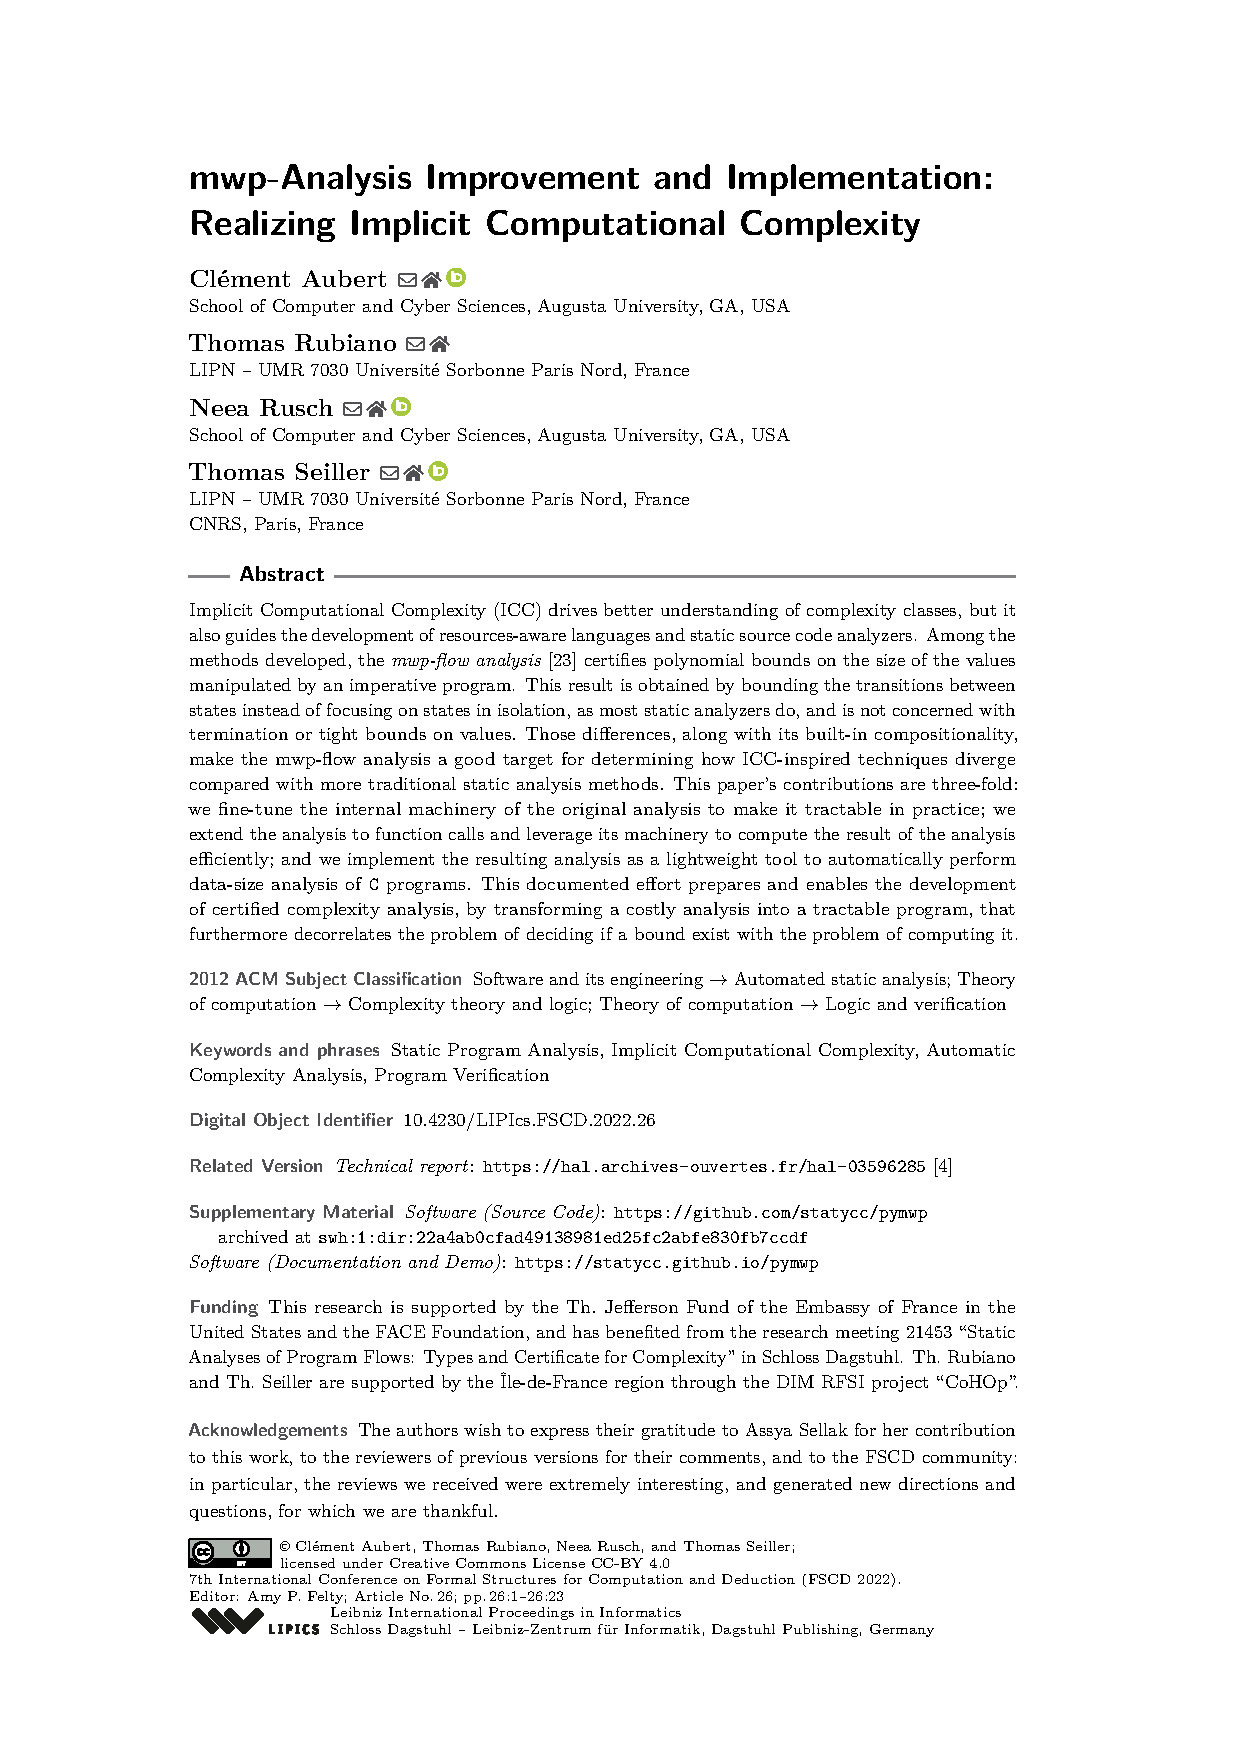
\includepdf[pages={1-},pagecommand={\thispagestyle{empty}%
\addtoindex{pymwp}{15}
\addtoindex{pymwp}{17}
\addtoindex{pymwp}{22}
\addtoindex{pymwp}{23}
\addtoindex{Coq}{16}
}]{res/pubs_fscd.2022.pdf}

\section{Distributing and Parallelizing Non-canonical Loops}\label{app:sec:vmcai}
\ainfo{\CTNT}{International Conference on Verification, Model Checking, and Abstract Interpretation, 2023}
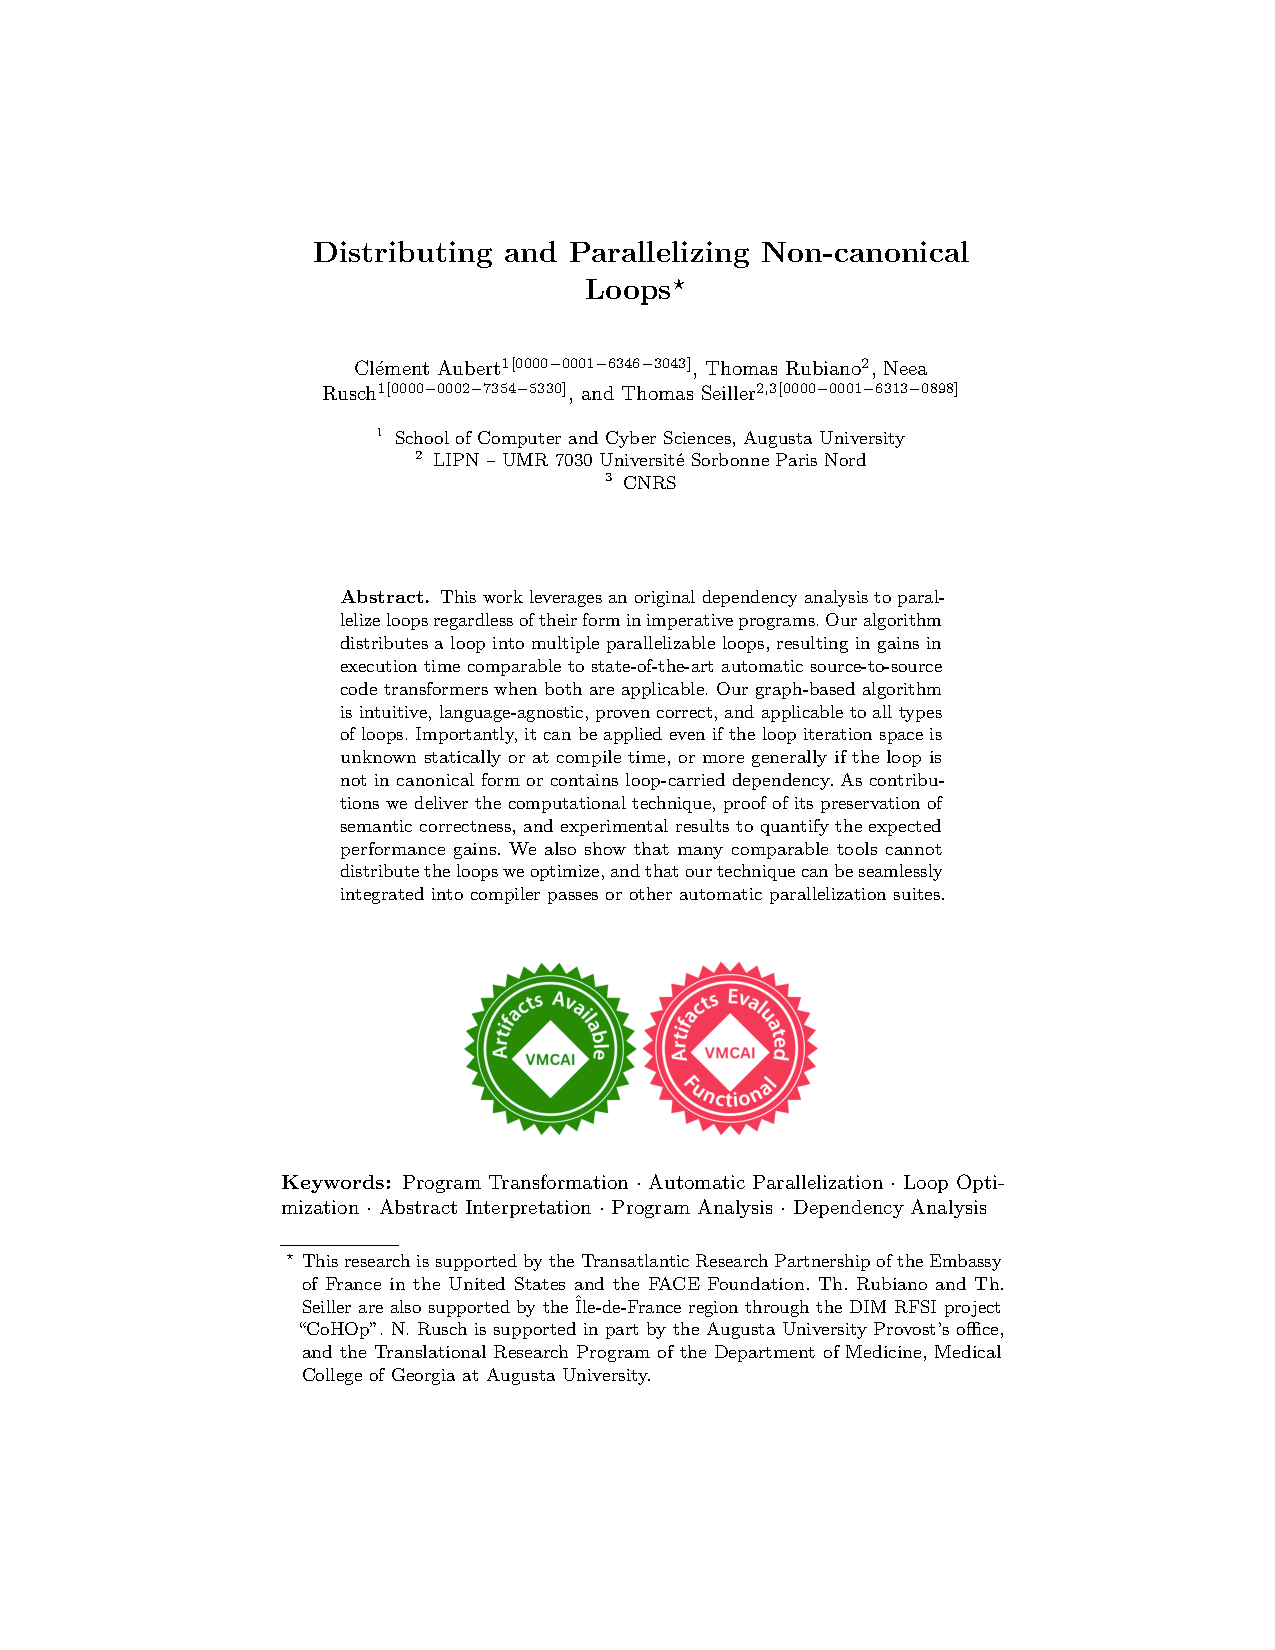
\includepdf[pages={1-},pagecommand={\thispagestyle{empty}%
\addtoindex{OpenMP}{2}
\addtoindex{OpenMP}{3}
\addtoindex{OpenMP}{4}
\addtoindex{OpenMP}{14}
\addtoindex{OpenMP}{15}
\addtoindex{OpenMP}{16}
\addtoindex{OpenMP}{18}
\addtoindex{OpenMP}{20}
\addtoindex{Polybench/C}{16}
\addtoindex{Polybench/C}{17}
\addtoindex{ROSE}{14}
\addtoindex{ROSE}{15}
\addtoindex{ROSE}{17}
\addtoindex{ROSE}{18}
\addtoindex{ROSE}{20}
}]{res/pubs_vmcai.2023.pdf}

\section{Tool User Guide for \enquote{pymwp: A Static Analyzer Determining Polynomial Growth Bounds}}\label{app:sec:tool-guide}
\ainfo{\CTNT}{Publication companion.}
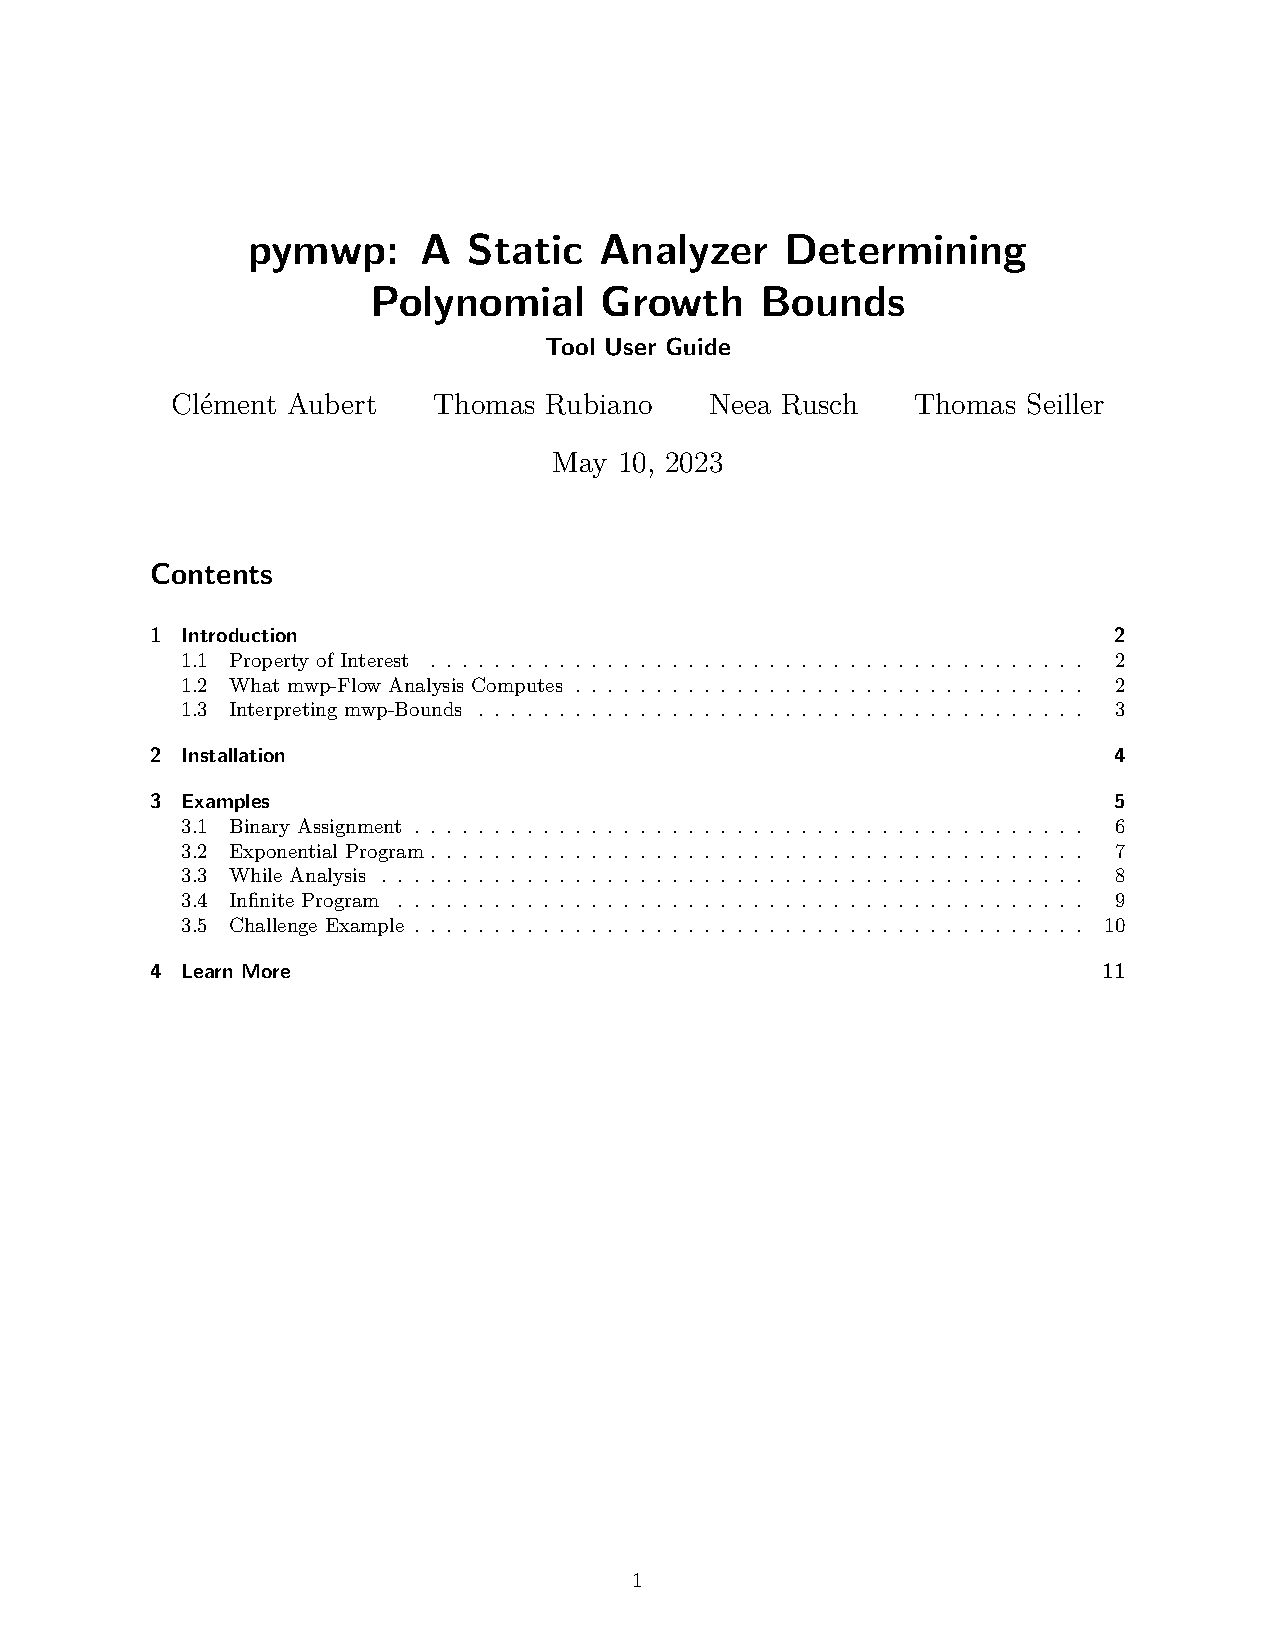
\includepdf[pages={1-},scale=0.9,offset=0 0.25in,pagecommand={\thispagestyle{empty}%
\addtoindex{pymwp}{1}
\addtoindex{pymwp}{2}
\addtoindex{pymwp}{4}
\addtoindex{pymwp}{5}
\addtoindex{pymwp}{6}
\addtoindex{pymwp}{7}
\addtoindex{pymwp}{8}
\addtoindex{pymwp}{9}
\addtoindex{pymwp}{10}
\addtoindex{pymwp}{11}
\addtoindex{mwp-bound}{3}
\addtoindex{mwp-bound}{8}
}]{res/pubs_pymwp_guide.pdf}

\section{Co-author Statements}\label{app:sec:coauth}
Include a detailed summary of the work performed by other authors on published or accepted manuscripts used in the thesis/dissertation.
Should additional authors (other than the candidate and the advisor) be listed on
one or more of the dissertation manuscripts, the candidate must provide a
detailed summary of the work performed by these other authors.
This summary may be provided in the “Acknowledgments” section of the dissertation.
Furthermore, a statement must be provided in the dissertation in which the
additional authors agree (by their signatures) with the candidate’s assessment of
their contribution to the manuscripts.

\clearpage\printnoidxglossary[type=\acronymtype]
\clearpage\printindex


\end{appendices}
\end{document}